% When submitting your files, remember to upload this *tex file, the pdf generated with it, the *bib file (if bibliography is not within the *tex) and all the figures.

% NB logo1.jpg is required in the path in order to correctly compile front page header %%%

\documentclass[utf8]{FrontiersinHarvard} % for articles in journals using the Harvard Referencing Style (Author-Date), for Frontiers Reference Styles by Journal—https://zendesk.frontiersin.org/hc/en-us/articles/360017860337-Frontiers-Reference-Styles-by-Journal
\usepackage{url,hyperref,lineno,microtype,subcaption}
%\usepackage[]{natbib, booktabs, graphicx, tabularx, makecell}
\usepackage{booktabs}
\usepackage{lscape, float, multirow, adjustbox}
\usepackage[T1]{fontenc}
\usepackage[onehalfspacing]{setspace}
\usepackage{graphicx} 

\linenumbers


% Leave a blank line between paragraphs instead of using \\


\def\keyFont{\fontsize{8}{11}\helveticabold }
\def\firstAuthorLast{Morris {et~al.}} %use et al only if is more than 1 author
\def\Authors{Joanna Morris\,$^{1,2,*}$, Emma Kealey\,$^{2,3}$, Frankie Greene\,$^{1,4}$, Joemari Pulido\,$^{2,5}$, Tess Rooney\,$^{2,6}$, Ethan Moore\, $^{2}$, Crismar Ramos-Marte\, $^{2}$, Natalia Alzate\,$^{2}$}
% Affiliations should be keyed to the author's name with superscript numbers and be listed as follows—Laboratory, Institute, Department, Organization, City, State abbreviation (USA, Canada, Australia), and Country (without detailed address information such as city zip codes or street names).
% If one of the authors has a change of address, list the new address below the correspondence details using a superscript symbol and use the same symbol to indicate the author in the author list.
\def\Address{$^{1}$School of Cognitive Science, Hampshire College, Amherst, MA, USA \\
	$^{2}$Department of Psychology, Providence College, Providence, RI, USA \\
	$^{3}$Department of Linguistics, University of Southern California, Los Angeles, CA, USA \\
	$^{4}$Oregon Health \& Science University and Portland State University School of Public Health, Portland, OR, USA \\
	$^{5}$Department of Cognitive, Linguistic \& Psychological Sciences, Brown University, Providence, RI, USA \\
	$^{6}$Columbia University School of Nursing, New York, NY, USA}
% The Corresponding Author should be marked with an asterisk
% Provide the exact contact address (this time including street name and city zip code) and email of the corresponding author
\def\corrAuthor{Joanna Morris}

\def\corrEmail{jmorris6@providence.edu}


\begin{document}
	\onecolumn
	\firstpage{1}
	
	\title[Running Title]{Reading skill and the time course of morphological processing: electrophysiological evidence for stage-specific modulation} 
	
	\author[\firstAuthorLast ]{\Authors} %This field will be automatically populated
	\address{} %This field will be automatically populated
	\correspondance{} %This field will be automatically populated
	
	\extraAuth{}% If there are more than 1 corresponding author, comment this line and uncomment the next one.
	%\extraAuth{corresponding Author2 \\ Laboratory X2, Institute X2, Department X2, Organization X2, Street X2, City X2 , State XX2 (only USA, Canada and Australia), Zip Code2, X2 Country X2, email2@uni2.edu}
	
	
	\maketitle
	
	
	
	
\begin{abstract}
		
		%%% Leave the Abstract empty if your article does not require one, please see the Summary Table for full details.
	\section{}
	Skilled reading of morphologically complex words depends on both high-quality lexical representations and sensitivity to morphological structure. However, we do not yet understand how these abilities shape the time course of morphological processing. In this study, event-related potentials (ERPs) and reaction times were recorded during a lexical decision task on morphologically complex words and nonwords; both varied in base frequency and family size, and nonwords additionally varied in morphological complexity. Individual differences were quantified via principal components analysis of vocabulary knowledge, spelling ability, and print exposure, yielding two orthogonal dimensions: Language Proficiency (LP) and Orthographic Sensitivity (OS). Behaviourally, response times were sensitive to base frequency and family size for words, and to morphological complexity for nonwords, while individual differences played a minor role: Orthographic Sensitivity showed a modest effect on response speed for nonwords only, and Language Proficiency showed no reliable effect. ERP measures revealed a richer picture. For familiar words, Orthographic Sensitivity primarily modulated the N250 base frequency effect, with a smaller Language Proficiency effect too; only Language Proficiency modulated the N400 base frequency effect. For novel morphologically complex forms, both Orthographic Sensitivity and Language Proficiency modulated the cost of morphological complexity at the N250. For both dimensions, the complexity cost shrank as skill increased and reversed direction at the highest skill levels. Because both dimensions were involved, this pattern qualifies the prediction that Orthographic Sensitivity alone governs early morphological parsing: instead, early parsing of novel forms appears to draw on reading skill more broadly. At the N400, a large morphological family made complex nonwords harder to process for readers lower in Language Proficiency, but this cost was absent for readers higher in Language Proficiency; Orthographic Sensitivity showed no comparable effect, giving the clearest evidence for the predicted dissociation between the two dimensions. Together these findings indicate that individual differences in reading skill are expressed chiefly in the dynamics of neural processing rather than in overt response times, and that the dissociation between orthographic and lexical-semantic profiles is clearest at the later stage where word meaning is accessed, while early morphological parsing of novel forms depends on both dimensions.
		
		
	\tiny
	\keyFont{ \section{Keywords:} morphological processing, individual differences, event-related potentials, N250, N400, lexical decision} %All article types—you may provide up to 8 keywords; at least 5 are mandatory.
\end{abstract}
	
	\section{Introduction}

	Reading is often described as "the process of gaining meaning from print" \citep[][p.~34]{raynerHowPsychologicalScience2001}. Getting from a visual word form to its meaning is not a single step: theories of language comprehension generally agree that this process unfolds across multiple stages, moving from sublexical orthographic analysis toward lexical and then semantic representation, though they disagree sharply about how many stages are involved and what mediates between them. English morphology offers a useful case for studying this question. English spelling maps unevenly onto sound, so phonological decoding alone cannot support fluent word recognition \citep{zieglerReadingAcquisitionDevelopmental2005, castlesHowDoesOrthographic2006}; but English morphology is comparatively regular, and words that share a base often show both consistent orthographic patterns and systematic semantic relationships (e.g., \textit{heal--health} share a stem; \textit{teacher}, \textit{baker}, and \textit{driver} share the agentive suffix \textit{-er}). Multi-morphemic words therefore provide a natural test case for asking how form-based and meaning-based information are related across the stages of word recognition.

	Readers vary considerably in how they navigate these stages \citep{perfettiReadingAbilityLexical2007, castlesHowDoesOrthographic2006, stanovichExposurePrintOrthographic1989}, and this variation offers a way to adjudicate between competing accounts of the stages themselves. If a lexical manipulation's effect depends systematically on the reader, that dependency is informative about what kind of representation the manipulation engages. The present study applies this logic to morphological processing. We examine two dissociable dimensions of reading skill, Orthographic Sensitivity (OS) and Language Proficiency (LP), in relation to two lexical variables long argued to index distinct levels of morphological representation: base frequency and morphological family size. By linking these individual differences to the N250 and N400 --- ERP components argued to index sequential stages from sublexical form analysis to semantic integration --- we ask whether the OS/LP dissociation tracks the form-based/meaning-based dissociation in real time. This approach is consistent with the major theoretical accounts of morphological processing: although these accounts disagree about mechanism, they converge on the prediction that base frequency and family size are temporally dissociable and should be differentially sensitive to a reader's orthographic versus semantic profile.

	To evaluate this prediction, four things need to be established before the study's specific aims can be stated. First, what base frequency and family size are each argued to index, and why competing theoretical accounts converge on expecting them to dissociate temporally. Second, how OS and LP emerge as dissociable dimensions of individual variation. Third, why the N250 and N400 are appropriate neural indices of the two processing stages in question. Fourth, what the dissociation between OS and LP predicts specifically for the parsing of novel morphological forms, building on prior evidence that affix-based and stem-based parsing mechanisms may operate concurrently.

	\subsection{Base Frequency and Morphological Family Size}

	Base frequency, the cumulative token frequency of a base morpheme across all its surface forms, and morphological family size, the number of distinct words sharing that base, both facilitate visual word recognition, and their effects are independent when appropriately controlled \citep{fordDerivationalMorphologyBase2010}. The two variables have been argued to index different levels of morphological representation: base frequency reflects the cumulative ease with which a base morpheme's orthographic form is processed across its surface variants, while family size reflects the breadth of meaning-level connections activated when a morphological base is encountered \citep{schreuderHowComplexSimplex1997, taftMorphologicalDecompositionReverse2004, taftRecognitionAffixedWords1979, dejongMorphologicalFamilySize2000, bertramEffectsFamilySize2000}.

	Current accounts of morphological processing disagree considerably about the architecture responsible for this pattern --- whether complex words are obligatorily decomposed into constituent morphemes, accessed via parallel whole-word and decompositional routes, or processed through learned form-to-meaning mappings without discrete morpheme representations at all \citep{schreuderModelingMorphologicalProcessing1995, dejongMorphologicalFamilySize2000, taft_lexical_1975, taftMorphologicalDecompositionReverse2004, rastleMorphologicalDecompositionBased2008, longtinMorphologicalDecompositionEarly2005, morrisSemanticTransparencyMasked2007, chuangDiscriminativeLearningLexicon}. Despite this disagreement, these accounts converge on a shared prediction: base frequency effects should arise earlier in processing than family size effects, reflecting a general precedence of form-level access over semantic integration. We return to how each account explains this precedence, and to what our results imply for adjudicating between them, in the General Discussion; here, the point is simply that the precedence itself is a point of theoretical consensus, which is what motivates using it to test the timing of OS and LP effects.

	\subsection{Orthographic Sensitivity and Language Proficiency as Dissociable Dimensions}

	Traditional models of word recognition typically characterise processing at the level of the skilled reader in general, abstracting over individual differences in favour of a uniform cognitive architecture. Yet readers do not differ along a single dimension of lexical skill. Andrews and colleagues \citep{andrewsIndividualDifferencesSkilled2012, andrewsMorphologicalPrimingStronger2013} showed that individual differences in orthographic and semantic knowledge are dissociable and predict distinct patterns of morphological processing: readers with a semantic profile, defined by relatively higher vocabulary than spelling ability, show robust priming for transparent morphological pairs but little priming for opaque or form-only pairs, particularly at longer latencies, while readers with an orthographic profile, defined by relatively higher spelling than vocabulary, show sustained priming for opaque pairs that is at least as strong as for transparent pairs. \citet{andrewsMorphologicalPrimingStronger2013} interpret this as evidence that readers differ not merely in overall processing efficiency but in the relative weight they assign to form-based versus meaning-based information during lexical access.

	The present study builds directly on this finding. If base frequency and family size index form-based and meaning-based aspects of lexical representation respectively, as established above, then readers who differ in their balance of orthographic and semantic processing should differ predictably in their sensitivity to each variable. To capture this variation continuously rather than as a categorical split, we derive two orthogonal dimensions, Language Proficiency and Orthographic Sensitivity, from a principal components analysis of vocabulary knowledge, spelling ability, and print exposure, following \citet{andrewsMorphologicalPrimingStronger2013}.

	\subsection{The N250 and N400 as Indices of Sequential Processing Stages}

	To track whether base frequency and family size effects emerge at distinct temporal stages, the present study uses two ERP components as dependent measures: the N250, an index of sublexical form processing, and the N400, an index of lexical-semantic integration. These components have been argued to reflect sequential stages in the cascade from orthographic decoding to meaning retrieval \citep{graingerWatchingWordGo2009}.

	The N250 is a negative-going deflection peaking at approximately 250~ms post-stimulus onset, proposed to reflect the stage at which sublexical orthographic representations are mapped onto higher-level form representations prior to full lexical access \citep{holcombTimeCourseVisual2006}. Evidence for this interpretation comes from its graded sensitivity to orthographic overlap in masked priming: amplitude is most attenuated for full identity repetitions, intermediate for primes sharing all but one letter, and largest for unrelated pairs \citep{holcombTimeCourseVisual2006, holcomb_exploring_2007}. The N250 is also sensitive to sublexical phonological overlap, with separable orthographic and phonological subcomponents \citep{graingerTimeCourseOrthographic2006}, consistent with its role as an early, form-based stage of processing.

	The N400 is a negative-going component peaking around 400~ms with a broad centro-parietal distribution \citep{kutasReadingSenselessSentences1980}. Its amplitude varies with semantic priming, cloze probability, and semantic richness, while remaining insensitive to physical and syntactic manipulations that leave meaning intact \citep{kutasThirtyYearsCounting2011}. In the present design, larger amplitudes are expected when a word's meaning is harder to integrate with the concurrently activated semantic information carried by its morphological family.

	The N250 and N400 are dissociable not only by topography --- frontal versus posterior \citep{holcombTimeCourseVisual2006} --- but by a double dissociation across priming types: lexical status modulates the N400 but not the N250, since N400 priming is restricted to real words and does not extend to pseudowords \citep{kiyonagaMaskedCrossmodalRepetition2007}, while the reverse holds for semantic relatedness, which modulates the N400 but produces no N250 effect \citep{graingerWatchingWordGo2009}. This pattern confirms that the two components index qualitatively distinct processing stages, ruling out the interpretation of the N250 as merely an early onset of the N400.

	\subsection{Affix-Led and Stem-Led Parsing}

	A recurring question in this literature is whether morphological decomposition is driven primarily by affix recognition or by stem activation. Affix-stripping accounts \citep{taft_lexical_1975, rastleMorphologicalDecompositionBased2008} propose that the affix is identified first and triggers decomposition, after which the stem is looked up in the lexicon. However, \citet{beyersmannEmbeddedStemPriming2016} found that high-proficiency readers showed embedded stem priming effects independent of affix status --- priming occurred even when the stem was followed by a non-affixal ending --- suggesting that stem activation in skilled readers need not be contingent on affix recognition, and that stem-based and affix-based mechanisms may operate concurrently.

	The present study tests this possibility directly. If Orthographic Sensitivity indexes the precision of sublexical orthographic representations, readers higher in Orthographic Sensitivity should show greater N250 sensitivity to the presence of a real versus pseudo-affix, consistent with affix-led parsing. If Language Proficiency instead indexes the depth and breadth of lexical-semantic knowledge in which stems are embedded, readers higher in Language Proficiency should show a distinct signature of stem-led parsing at the same stage. Because Beyersmann et al.'s proficiency measure was not decomposed into orthographic and lexical-semantic components, it is unclear from their data alone which mechanism their finding reflects. The present design, with Orthographic Sensitivity and Language Proficiency measured as separate dimensions, is positioned to address this question directly.

	\subsection{Aims and Predictions}

	The present study has two complementary aims. The first is to establish whether base frequency and morphological family size exert their effects at distinct temporal stages of visual word recognition. The second, and primary, aim is to examine whether Orthographic Sensitivity and Language Proficiency modulate these effects selectively, at the processing stages where each variable is predicted to operate.

	The core prediction is a pattern of component-specific modulation: Orthographic Sensitivity should modulate base frequency effects at the N250, while Language Proficiency should modulate family size effects at the N400. If this pattern is observed, it would constitute direct electrophysiological evidence that the distinction between form-based and meaning-based morphological processing is a real axis of variation in the reading system, not merely a property of competing computational models. If instead both variables are modulated by the same individual difference dimension at the same stage, this would suggest that the two effects are less dissociable than current multi-stage accounts propose.

	The first analysis examines this prediction in real word recognition. Because word stimuli were not matched across morphological variables, base frequency, family size, and morphological complexity are treated as continuous predictors in a regression framework for reaction times; for ERP data, items were median-split into high and low groups separately for base frequency and family size. The two measures therefore carry somewhat different inferential weight: the RT regression speaks to the independent continuous contributions of each variable, while the ERP analyses speak to the direction and timing of effects at the extremes of each variable's distribution.

	The second analysis examines whether these modulations generalise to novel morphological structure, using morphologically complex nonwords. Morphologically structured nonwords (e.g., \textit{gasful}: real stem + real affix) were compared against matched controls (e.g., \textit{gasfil}: real stem + pseudoaffix), holding stem identity constant while manipulating suffix legitimacy. Because these items have no stored whole-word representations, they place maximal pressure on the system's generalisation mechanism and allow stem-level variables to be examined independently of whole-word familiarity. Orthographic Sensitivity is predicted to modulate early N250 responses to the suffix contrast, consistent with affix-led parsing: readers with more precise representations of real suffix forms should show greater N250 sensitivity to the distinction between real and pseudo-suffixes. Language Proficiency, building on the stem-led parsing possibility developed above, is predicted to modulate N250 responses through a distinct mechanism, and to predict later N400 sensitivity to whether a nonword's stem belongs to a large or productive morphological family, since it is this family membership that determines the richness of the semantic activation the form can support.

	
	\section{Methods}
	
	\subsection{Materials}
	
	All stimulus items---200 nonword words, 100 morphologically complex words, and 100 monomorphemic filler items---were adapted from \citet{sawiIndividualDifferencesSensitivity2016}. The 200 nonwords, were constructed to manipulate morphological structure while controlling surface form. In the \textit{complex nonword} condition, existing English base words (e.g., \textit{gas}) were combined with existing derivational suffixes (e.g., \textit{gasful}), to yield 100 morphologically plausible complex nonwords. Each combination was syntactically legal and reflected common English derivational patterns. A total of 16 suffixes were used, each attached to four different stems.
	
	In the \textit{simple nonword} condition, the same base words as in the complex non-word condition were combined with non-suffix endings that were orthographically similar to the real suffixes used in the complex condition but did not constitute valid morphemes, to yield 100 orthographically plausible simple non-words. These pseudoaffix endings were created by changing the central letter of each suffix (e.g., \textit{gasful}–\textit{gasfil}), preserving length and orthographic neighborhood characteristics while eliminating morphological structure. Thus each complex non-word had an orthographically matched simple counterpart.
	
	Because the same base appeared in both the simple and complex conditions, the experimental nonwords were distributed across two lists such that no participant encountered the same base more than once. In addition to the experimental nonwords, the stimulus set included 100 monomorphemic fillers (50 real words and 50 nonwords) to balance lexical status and reduce predictability. The experimental stimuli were drawn from \citet{sawiIndividualDifferencesSensitivity2016}.
	Estimates of cumulative base (root) frequency, surface frequency, and morphological family size were obtained from the CELEX lexical database. Morphological family size was calculated by identifying all morphologically related forms sharing the same base (e.g., \textit{calculate}, \textit{calculable}, \textit{calculation}, \textit{calculator}). Following prior work \citep[e.g.,][]{dejongMorphologicalFamilySize2000, dejongProcessingRepresentationDutch2002}, both compounds (e.g., \textit{WATCHTOWER}) and hyphenated compounds (e.g., \textit{CHECK-IN}) were included, as they contribute to morphological connectivity within the lexicon. Base frequency was computed by summing the lemma frequencies of all confirmed family members.
	
	The morphologically complex word stimuli consisted of 100 semantically transparent words with exclusively productive suffixes, a subset of the item set from \citet{fordDerivationalMorphologyBase2010} selected by \citet{sawiIndividualDifferencesSensitivity2016}. The words varied in base and surface frequency as well as in morphological family size.
	
	For reaction time analyses, all lexical and individual-difference variables were treated as continuous predictors to preserve information and maximize statistical power. In contrast, ERP analyses were conducted on condition-averaged waveforms to improve signal-to-noise ratio; as a result, item-level predictors such as base frequency and family size were operationalized as categorical condition factors rather than continuous trial-level covariates. This distinction reflects standard practice in ERP research and aligns the statistical treatment of predictors with the structure of the underlying data.
	
	\subsection{Individual Differences and Grouping Variables}
	
	To quantify individual differences in linguistic experience and orthographic knowledge, participants completed three standardized measures---the Nelson–Denny Vocabulary Test \citep{brownNelsonDennyReadingTest1993}, a spelling task adapted from \citet{sawiIndividualDifferencesSensitivity2016}, and the Author Recognition Test (ART; \citealt{stanovichExposurePrintOrthographic1989}). Scores on these measures were moderately correlated ($r$s = .29–.51, all $p < .02$), indicating partially overlapping but dissociable components of lexical experience.
	
	To capture the shared and distinct variance among these measures, we conducted a principal components analysis (PCA) on standardized (z-scored) vocabulary, spelling, and ART scores. PCA was selected to derive orthogonal dimensions of individual differences without imposing a priori weighting or categorical group boundaries. Two components had eigenvalues greater than 1, jointly accounting for 83.5\% of the total variance (58.0\% for Dimension~1 and 25.5\% for Dimension~2).
	
	Component loadings (Table~\ref{tab:pca_loadings}) indicated that Dimension~1 loaded most strongly on vocabulary and print exposure (ART), with a secondary contribution from spelling accuracy, and was interpreted as indexing \textit{Language Proficiency}. Dimension~2 loaded most strongly on spelling accuracy, with weaker and oppositely signed contributions from vocabulary and ART, and was interpreted as indexing \textit{Orthographic Sensitivity}:
	
	\begin{itemize}
		\item[-] \textit{Dimension~1 (Language Proficiency)}: vocabulary (.82), ART (.81), spelling (.65)
		\item[-] \textit{Dimension~2 (Orthographic Sensitivity)}: spelling (.76), vocabulary ($- .29$), ART ($- .32$)
	\end{itemize}
	
	The two components were statistically independent ($r \approx 0$), supporting their interpretation as orthogonal dimensions of reading-related skill. These continuous component scores were used as predictors in all behavioral and ERP analyses.
	
	
	\begin{table}[ht]
		\centering
		\caption{PCA loadings and variance explained for the three lexical-experience measures.}
		\label{tab:pca_loadings}
		\begin{tabular}{lcc}
			\toprule
			\textbf{Measure} & \textbf{\shortstack{Dimension~1 \\ (Language Proficiency)}} & \textbf{\shortstack{Dimension~2 \\ (Orthographic Sensitivity)}} \\
			\midrule
			Vocabulary (z\_vcb) & 0.82 & $-0.29$ \\
			Spelling (z\_spl) & 0.65 & 0.76 \\
			Author Recognition Test (z\_art) & 0.81 & $-0.32$ \\
			\midrule
			\textit{Eigenvalue} & 1.74 & 0.76 \\
			\textit{Variance explained (\%)} & 58.0 & 25.5 \\
			\bottomrule
		\end{tabular}
	\end{table}
	
	\subsection{Statistical Analyses}
	
	The analyses are organized around the study’s primary theoretical aim, determining whether Orthographic Sensitivity and Language Proficiency differentially modulate the timing and nature of morphological processing. We predicted that Orthographic Sensitivity would primarily modulate early, form-based processing indexed by the N250, while Language Proficiency would primarily modulate later semantic integration indexed by the N400. The behavioral and ERP results are reported separately for words and nonwords, followed by a summary that evaluates these predictions against the obtained pattern.
	
	\subsubsection{Behavioral Data (Reaction Times)}
	Reaction time (RT) analyses were conducted on correct responses only. RTs were log-transformed to reduce positive skew and to better meet model assumptions of normality and homoscedasticity. Separate analyses were conducted for word and nonword trials: for words, base frequency and family size were the primary morphological predictors; for nonwords, morphological complexity (real vs. pseudo-suffix) was the key manipulation, with base frequency and family size included as covariates (see Aims and Predictions).
	
	RTs were analyzed using linear mixed-effects models fit with the \texttt{lme4} package \citep{batesFittingLinearMixedeffects2015} in R \citep{rcoreteamLanguageEnvironmentStatistical2026}. All models included random intercepts for participants and items, and random slopes for within-participant predictors where supported by the data. Continuous lexical predictors (log base frequency and log family size) were mean-centered and scaled prior to analysis. Individual-difference measures—Orthographic Sensitivity and Language Proficiency—were entered as continuous predictors corresponding to standardized PCA scores.
	
	For word trials, models tested the effects of base frequency, family size, Orthographic Sensitivity, and Language Proficiency, as well as interactions between Orthographic Sensitivity and lexical familiarity measures. For nonword trials, models additionally included morphological complexity (simple vs. complex) as a categorical predictor and tested whether complexity effects were modulated by individual differences. Treatment (reference) coding was used for categorical predictors in RT analyses. Model significance was assessed using Type III tests with Satterthwaite-approximated degrees of freedom. Fixed-effect estimates are reported alongside model-based estimated marginal means where relevant. Means are reported in milliseconds following back-transformation from the log scale used in analysis.
	
	\subsubsection{ERP Data}
	
	For word stimuli, ERP trials were averaged separately according to median splits on base frequency and morphological family size, enabling separate analyses of each variable at the N250 and N400. For nonword stimuli, trials were averaged according to a median split on morphological family size. 
	
	The choice of primary item-level variable differed across stimulus types for theoretically motivated reasons. For word stimuli, base frequency was treated as the primary morphological variable of interest in the ERP analyses, because it indexes the strength of the stored lexical representation, that is, how well-entrenched the stem form is in the reader's mental lexicon as a function of accumulated encounter frequency. This makes it the most theoretically relevant item-level variable for examining individual differences in how stored lexical representations are accessed and processed at each ERP stage. For nonword stimuli, morphological family size was treated as the primary item-level variable, because nonwords have no stored whole-word representations and processing must rely on stem-level morphological properties. Family size indexes the richness of the stem's morphological neighbourhood, that is, how many distinct derived words share the stem and reinforce its semantic core, and is therefore the most theoretically relevant variable for examining how morphological family information is recruited when processing a novel form in the absence of whole-word familiarity. This asymmetry between stimulus types reflects the distinct theoretical roles of the word and nonword analyses; words examine the time course of stored lexical representation access, while nonwords examine morphological generalisation to novel forms.
	
	Within the nonword analyses, family size's statistical role further differed across the two time windows: at the N400 it was a primary predictor of theoretical interest, entering into three-way interactions with Morphological Complexity and each individual difference dimension; at the N250 it was retained as a covariate to reduce item-level variance rather than as a predictor of theoretical interest in its own right. Because base frequency and family size are properties of the stem shared across both members of each complexity pair (e.g., \textit{gasful} and \textit{gasfil} share the same stem), neither variable could confound the complexity manipulation. Family size was preferred over base frequency as the N250 covariate on empirical grounds: preliminary model comparisons indicated that family size accounted for substantially more item-level variance in the nonword N250 data (residual variance: 4.07 vs.\ 27.47). The pattern of interactions reported below was equivalent in direction when base frequency was used as the covariate instead.
	
	ERP analyses were conducted on mean amplitudes computed from condition-averaged waveforms. Separate datasets were constructed for words and nonwords, and analyses were conducted independently for the N250 and N400 time windows. Because ERP amplitudes were derived from condition-level averages rather than trial-level data, morphological predictors in ERP analyses were treated as categorical condition factors rather than continuous covariates.
	
	ERP amplitudes were analysed using linear mixed-effects models. For word stimuli, separate models were fit for base frequency and family size, each entered as the primary morphological predictor along with Orthographic Sensitivity, Language Proficiency, and their interaction with the morphological predictor. The non-interacting individual difference dimension was included as a covariate in each model: Language Proficiency was a covariate in the N250 models, and Orthographic Sensitivity was a covariate in the N400 models. For nonword stimuli, model structure differed across time windows to reflect the distinct role of family size at each stage. At the N250, models included fixed effects of Morphological Complexity, Orthographic Sensitivity, Language Proficiency, interactions between Complexity and each individual difference dimension, and Morphological Family Size as a covariate. At the N400, a single symmetric model was fit including fixed effects of Morphological Complexity, Morphological Family Size, Language Proficiency, Orthographic Sensitivity, and all two- and three-way interactions among Complexity, Family Size, and each individual difference dimension separately. This symmetric structure permitted direct comparison of the roles of LP and OS in modulating the joint influence of morphological complexity and family size on N400 amplitude, providing a formal test of the predicted dissociation between the two dimensions rather than assuming it in the model specification. All models included random intercepts for participants and for electrode site nested within participant, allowing baseline amplitude differences across electrodes to be modelled while preserving the spatial structure of the data.
	
	Categorical predictors in ERP analyses were effect-coded (sum-to-zero coding), such that model intercepts represent grand mean amplitudes and main effects reflect average effects across conditions. Orthographic Sensitivity and Language Proficiency were entered as continuous, mean-centred predictors. Time window was not included as a factor in the models; instead, separate models were fit for the N250 and N400 to preserve component-specific interpretation.
	
	Statistical significance of fixed effects was assessed using Type III $F$-tests with Satterthwaite-approximated degrees of freedom as implemented in the \texttt{lmerTest} package \citep{kuznetsovaLmerTestPackageTests2017}. Where higher-order interactions involving individual-difference measures were significant, follow-up analyses were conducted using estimated marginal means (\texttt{emmeans}). Interactions involving Orthographic Sensitivity and Language Proficiency were probed by estimating contrasts across the observed range of each dimension in the sample, allowing direct tests of whether morphological effects differed as a function of reader skill and characterising the full extent of any reversals across the individual difference continua.
	
	\subsubsection{Model Estimation and Inference}
	All mixed-effects models were fit using restricted maximum likelihood estimation. To ensure stable convergence, models were estimated using the BOBYQA optimizer. Continuous predictors were centered to facilitate interpretation of interaction terms and model intercepts. For predictors with one degree of freedom, F-tests from the analysis-of-variance tables are mathematically equivalent to squared t-tests from model summaries; all inferential conclusions are therefore invariant to the choice of reporting format. Across all analyses, inferential emphasis was placed on theoretically motivated interactions rather than exhaustive post hoc comparisons. Follow-up contrasts were conducted only where warranted by significant interactions and were limited to tests directly addressing the study’s hypotheses. Estimated marginal means and confidence intervals were obtained using the \texttt{emmeans} package \citep{lenthEmmeansEstimatedMarginal2026}; confidence intervals are based on asymptotic approximation, which is appropriate given the sample size.
	
	\section{Results}
	
	The analyses are organised around two complementary sources of evidence bearing on the study's primary theoretical aim --- determining how Orthographic Sensitivity and Language Proficiency jointly and differentially modulate the timing and nature of morphological processing. Reaction time models included individual difference measures as main effects only, reflecting the theoretical framing of behavioural responses as indices of overall processing efficiency. Interactions between morphological variables and individual differences were examined in the ERP models, where the temporal resolution of the N250 and N400 allows these effects to be attributed to specific processing stages. Because the Introduction treats Orthographic Sensitivity and Language Proficiency as parallel, equally weighted dimensions, both were fully crossed with each other and with the lexical variable of interest in every ERP model, rather than one dimension being assigned a priori as the primary moderator at a given component; this allows the data, rather than the model specification, to determine whether and where the two dimensions' influence diverges. Results are reported separately for words and nonwords. For each stimulus type, behavioural results are presented first, followed by ERP results organised by component, N250 then N400, reflecting the temporal sequence of morphological processing. This organisation reflects the distinct theoretical roles of the two stimulus types --- the word analyses examine the time course of base frequency and family size effects in stored lexical representations, while the nonword analyses examine whether morphological sensitivity generalises to novel forms and whether individual differences modulate that generalisation. Within each section, the pattern of effects is evaluated against the predictions derived from morpho-orthographic decomposition accounts and the Lexical Quality Hypothesis, with particular attention to whether individual-difference sensitivity is shared across both dimensions at the earlier component and narrows toward one dimension at the later component.
	
	Table~\ref{tab:models} summarises the fixed effects and interaction terms included in each model. For word stimuli, separate ERP models were run for base frequency and family size at each component, with Orthographic Sensitivity, Language Proficiency, and the lexical variable of interest fully crossed in a three-way interaction; neither individual difference dimension was demoted to a covariate in these models, since both are treated as theoretically parallel. For nonword stimuli, the N250 and N400 models each fully crossed Orthographic Sensitivity, Language Proficiency, and family size; morphological complexity was crossed individually with each of these three terms but was not required to enter a four-way interaction with all three simultaneously, a simplification confirmed by an omnibus check reported below. Two additional nonword models tested base frequency in place of family size at each component, to establish whether the observed three-way interactions were specific to family size; these specificity-check models are reported as null results rather than as primary findings. Reaction time models included individual difference measures as main effects only, reflecting the theoretical framing of behavioural responses as indices of overall processing efficiency rather than processing architecture.
	
	\begin{table}[h!]
		\centering
		\small
		\renewcommand{\arraystretch}{1.4}
		\caption{Summary of linear mixed-effects models. OS = Orthographic Sensitivity; LP = Language Proficiency; BF = Base Frequency; FS = Family Size; Cmplx = Morphological Complexity. All models fit by REML using the \texttt{bobyqa} optimizer. Degrees of freedom estimated using Satterthwaite's method. RE = random effects; Subj = participant; Elec = electrode site nested within participant. The Interaction(s) column lists the highest-order term of theoretical interest for each model; all lower-order interaction and main-effect terms implied by the listed term were also included. $^\dagger$ = three-way interaction with the lexical variable of interest was tested but non-significant; the interaction listed is the highest-order term that survived. $^\ddagger$ = specificity-check model substituting base frequency for family size, to confirm that the corresponding primary three-way interaction is family-size-specific rather than a general property of the design; the listed interaction was tested and found non-significant.}
		\label{tab:models}
		\begin{tabular}{p{1.6cm} p{1.2cm} p{1.3cm} p{3.8cm} p{3.2cm} p{2.5cm}}
			\toprule
			\textbf{Stimulus} & \textbf{Outcome} & \textbf{Variable} & 
			\textbf{Fixed effects} & \textbf{Interaction(s)} & 
			\textbf{RE structure} \\
			\midrule
			Words & RT & BF + FS & BF, FS, OS, LP & None & Subj, Item \\
			Words & N250 & BF & BF, OS, LP & BF $\times$ OS $\times$ LP & Subj, Elec/Subj \\
			Words & N250 & FS & FS, OS, LP & FS $\times$ OS $\times$ LP & Subj, Elec/Subj \\
			Words & N400 & BF$^\dagger$ & BF, OS, LP & BF $\times$ LP & Subj, Elec/Subj \\
			Words & N400 & FS$^\dagger$ & FS, OS, LP & None & Subj, Elec/Subj \\
			Nonwords & RT & BF + FS & Cmplx, BF, FS, OS, LP & None & Subj (Cmplx slope), Item \\
			Nonwords & N250 & FS & Cmplx, OS, LP, FS & Cmplx $\times$ OS, Cmplx $\times$ LP, OS $\times$ LP $\times$ FS & Subj, Elec/Subj \\
			Nonwords & N250 & BF$^\ddagger$ & Cmplx, OS, LP, BF & OS $\times$ LP $\times$ BF & Subj, Elec/Subj \\
			Nonwords & N400 & FS & Cmplx, FS, LP, OS & Cmplx $\times$ OS, Cmplx $\times$ LP, Cmplx $\times$ FS, FS $\times$ LP, OS $\times$ LP $\times$ FS & Subj, Elec/Subj \\
			Nonwords & N400 & BF$^\ddagger$ & Cmplx, BF, LP, OS & Cmplx $\times$ BF $\times$ LP & Subj, Elec/Subj \\
			\bottomrule
		\end{tabular}
	\end{table}
	
	The model structure reflected in Table~\ref{tab:models} warrants brief explanation. Individual difference terms (OS, LP) were fully crossed with each other and with the lexical variable of interest in every confirmatory model, since both dimensions are treated as theoretically parallel; higher-order interactions with the structural manipulation present in the nonword stimuli (morphological complexity) were tested as a follow-up specificity or robustness check rather than included in the confirmatory model, given the added parameters relative to sample size. For word stimuli, separate ERP models were run for base frequency and family size at each time window, reflecting the fact that these variables were operationalised as separate median-split factors in distinct datasets. At both the N250 and the N400, Orthographic Sensitivity and Language Proficiency were fully crossed with each other and with the lexical variable of interest, yielding a three-way interaction term at each component. Neither individual difference dimension was assigned a priori as the primary moderator at either component, nor was either dimension demoted to a covariate: the Introduction treats OS and LP as theoretically parallel, equally weighted dimensions, and there is no principled basis for building an asymmetric interaction structure into the models themselves. This structure allows the data to determine whether, and at which component, the two dimensions' modulation of base frequency and family size converges or diverges.

	For word stimuli, the three-way interaction was significant at the N250 for both base frequency and family size, but not at the N400 for either variable, where only lower-order terms survived (reported below); these outcomes are reported directly in the corresponding rows of Table~\ref{tab:models} rather than treated as confirmatory versus exploratory in the model specification itself. For nonword stimuli, an additional check was conducted before finalising the confirmatory models: a fully saturated model crossing Morphological Complexity with Orthographic Sensitivity, Language Proficiency, and family size simultaneously was fit at each component to test whether Complexity needed to enter a four-way interaction with both individual difference dimensions and the lexical variable. The four-way term was non-significant at both components (N250: $p = .439$; N400: $p = .510$), justifying its exclusion from the confirmatory models reported here, in which Complexity is instead crossed individually with each of Orthographic Sensitivity, Language Proficiency, and family size.

	For nonword stimuli, family size was fully crossed with Orthographic Sensitivity and Language Proficiency at both the N250 and the N400, rather than entered as a covariate at the N250 as in an earlier model specification; the three-way Orthographic Sensitivity $\times$ Language Proficiency $\times$ Family Size interaction was significant at both components. Morphological Complexity was crossed individually with Orthographic Sensitivity, Language Proficiency, and family size, consistent with the theoretically motivated affix-led/stem-led prediction developed in the Aims and Predictions section, without requiring the four-way term ruled out above. Two additional nonword models substituted base frequency for family size at each component, retaining the same crossed structure with Orthographic Sensitivity and Language Proficiency, in order to establish whether the three-way interaction observed for family size was specific to that variable rather than a general property of the nonword design. At neither component did the corresponding base-frequency three-way reach significance, supporting the specificity of the family-size effect; these models are reported in Table~\ref{tab:models} as null specificity checks rather than as primary findings.
	
	\subsection{Words}
	
	\paragraph*{Words RT}
	Reaction times (RTs) for correct lexical decisions to word stimuli were analyzed using a linear mixed-effects model with fixed effects of Base Frequency, Family Size, Orthographic Sensitivity (OS), and Language Proficiency (LP). The model included random intercepts for participants and items. The analysis revealed robust main effects of item-level lexical familiarity. As base frequency increased, recognition times decreased, $\beta = -0.017$, $SE = 0.005$, $t(100.97) = -3.66$, $p < .001$, $\eta^2_p = .12$. Similarly, words from larger morphological families elicited faster responses than those from smaller families, $\beta = -0.013$, $SE = 0.005$, $t(93.59) = -2.64$, $p = .010$, $\eta^2_p = .07$. Orthographic Sensitivity showed a marginal trend toward faster overall response times, $\beta = -0.035$, $SE = 0.019$, $t(63.84) = -1.85$, $p = .069$, $\eta^2_p = .05$. Language Proficiency did not exert a reliable main effect on RTs, $\beta = 0.012$, $SE = 0.012$, $t(63.97) = 0.94$, $p = .35$. The model explained 3.3\% of the variance via fixed effects ($R^2_{\mathrm{marginal}} = .033$) and 41.7\% overall ($R^2_{\mathrm{conditional}} = .417$). These findings indicate that word recognition speed is driven primarily by item-level lexical familiarity; Orthographic Sensitivity shows only a marginal and unstable influence on overall response efficiency and does not selectively modulate morphological effects on response times. (See Figure \ref{fig:fig1a})
	
	\begin{figure}[htbp]
		\centering
		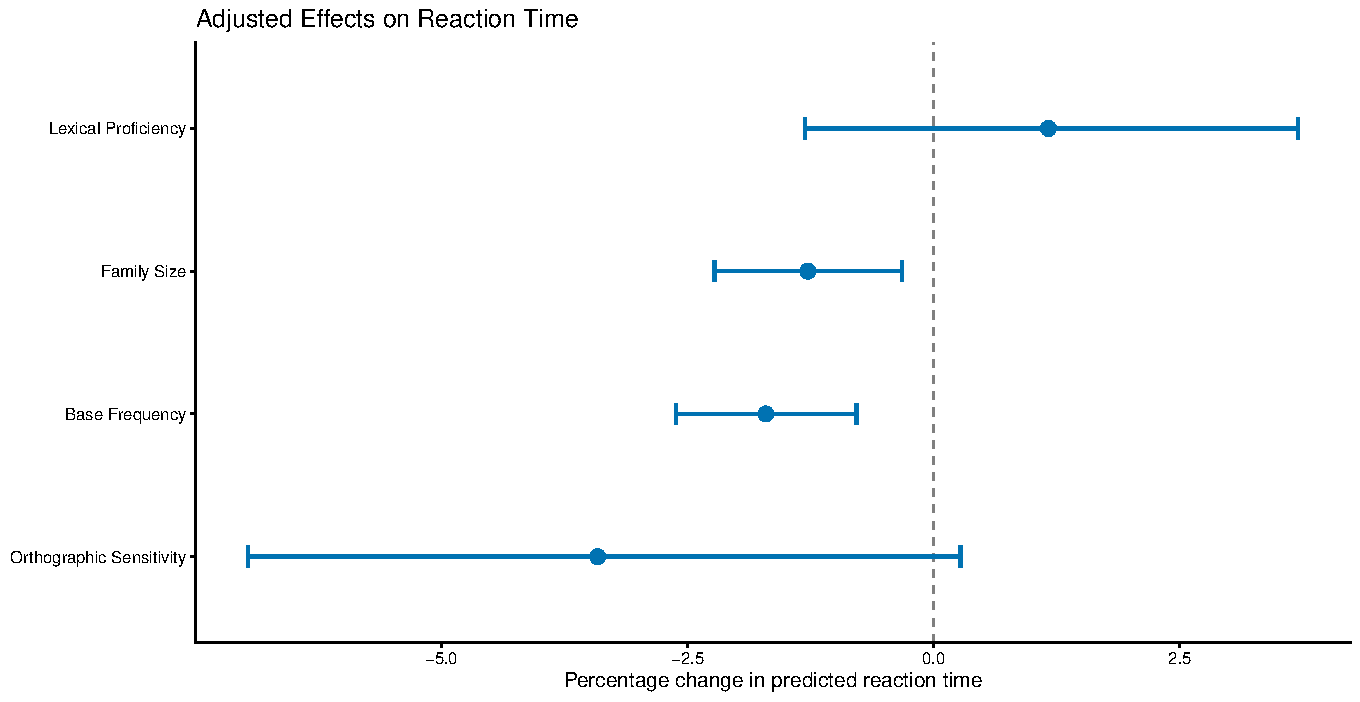
\includegraphics[width=0.5\textwidth]{Figure 1a Words_RT_coefficient_plot}
		\caption{ Estimated regression coefficients and 95\% confidence intervals for subject the variables Lexical Proficiency, Orthographic Sensitivity,and the item variables  Morphological Family Size and Base Frequeny. Point estimates (dots) show the effect size for each predictor variable, with horizontal whiskers representing 95\% confidence intervals. The vertical dashed line marks the null effect at zero. Variables with intervals not crossing zero are statistically significant.}
		\label{fig:fig1a}
	\end{figure}
	
	\paragraph*{Words N250: Base Frequency}
	Mean N250 amplitudes for word stimuli were analysed using a linear mixed-effects model with fixed effects of Base Frequency (high vs.\ low), Orthographic Sensitivity (OS), Language Proficiency (LP), and their full three-way interaction. The model included random intercepts for participants and for electrode site nested within participant. The analysis revealed a significant main effect of Base Frequency --- words from higher-frequency bases elicited more negative N250 amplitudes than words from lower-frequency bases, $\beta = -0.326$, $SE = 0.099$, $t(1616) = -3.28$, $p = .001$, $\eta^2_p = .007$. Neither Orthographic Sensitivity, $\beta = 0.538$, $SE = 0.522$, $t(56) = 1.03$, $p = .307$, nor Language Proficiency, $\beta = -0.567$, $SE = 0.382$, $t(56) = -1.49$, $p = .143$, yielded reliable main effects.

	Critically, the three-way interaction between Base Frequency, Orthographic Sensitivity, and Language Proficiency was significant, $\beta = -0.537$, $SE = 0.108$, $t(1616) = -4.97$, $p < .0001$, $\eta^2_p = .02$, and was robust to the exclusion of the single participant with the most extreme Language Proficiency score (2.55 SD above the sample mean; $\beta = -0.534$, $t = -4.92$, $p < .0001$ with that participant excluded). Rather than a simple amplification of the Base Frequency effect by one dimension, the interaction took the form of a crossover: the direction of the Base Frequency effect depended jointly on OS and LP. Within the primary reporting range of $\pm 1.5$ SD on both dimensions, the Language Proficiency slope of the Base Frequency effect reversed sign as OS moved from low to high --- significantly negative at low OS ($\beta = -0.93$, $SE = 0.17$, $t(1616) = -5.39$, $p < .0001$), non-significant near the mean of OS ($\beta = -0.13$, $SE = 0.08$, $t(1616) = -1.59$, $p = .113$), and significantly positive at high OS ($\beta = 0.68$, $SE = 0.19$, $t(1616) = 3.58$, $p < .0001$). The mirror-image contrast, examining the OS slope of the Base Frequency effect across LP, showed the same pivot within this range: non-significant at low LP ($\beta = -0.36$, $SE = 0.20$, $t(1616) = -1.82$, $p = .068$) and significantly positive from the mean of LP upward ($\beta = 0.44$, $SE = 0.11$, $t(1616) = 4.01$, $p < .0001$ at LP $= 0$; $\beta = 1.25$, $SE = 0.20$, $t(1616) = 6.39$, $p < .0001$ at LP $= +1.5$ SD), consistent with a single underlying crossover surface (see Figure~\ref{fig:fig1b}, panel A).

	The same direction of crossover was evident, more tentatively, among the small number of participants beyond $\pm 1.5$ SD on both dimensions simultaneously; these joint-extreme corners are sparsely populated and are shown as the faded, dashed extensions in Figure~\ref{fig:fig1b} rather than reported as separate statistical tests. The model explained 1.8\% of variance via fixed effects ($R^2_{\mathrm{marginal}} = .018$) and 80.5\% overall ($R^2_{\mathrm{conditional}} = .805$).

	\paragraph*{Words N250: Family Size}
	A parallel model examined mean N250 amplitudes as a function of Family Size (large vs.\ small), Orthographic Sensitivity, Language Proficiency, and their full three-way interaction, with the same random-effects structure as the base frequency model above. The analysis revealed a significant main effect of Family Size --- words from larger morphological families elicited less negative (more positive) N250 amplitudes than words from smaller families, $\beta = 0.312$, $SE = 0.058$, $t(1616) = 5.37$, $p < .0001$, $\eta^2_p = .02$. Neither Orthographic Sensitivity, $\beta = 0.263$, $SE = 0.257$, $t(56) = 1.02$, $p = .312$, nor Language Proficiency, $\beta = -0.295$, $SE = 0.188$, $t(56) = -1.57$, $p = .123$, yielded reliable main effects.

	As with base frequency, the three-way interaction between Family Size, Orthographic Sensitivity, and Language Proficiency was significant, $\beta = -0.282$, $SE = 0.063$, $t(1616) = -4.46$, $p < .0001$, $\eta^2_p = .01$, and took the form of a crossover rather than a simple amplification. Within the primary reporting range of $\pm 1.5$ SD, the Language Proficiency slope of the Family Size effect reversed sign as OS moved from low to high --- significantly negative at low OS ($\beta = -0.33$, $SE = 0.10$, $t(1616) = -3.23$, $p = .001$), and significantly positive at high OS ($\beta = 0.52$, $SE = 0.11$, $t(1616) = 4.69$, $p < .0001$). Unlike the base frequency crossover, this reversal was already detectable near the mean of OS: the Language Proficiency slope was significantly positive at OS $= 0$ ($\beta = 0.10$, $SE = 0.05$, $t(1616) = 2.01$, $p = .044$), indicating that the pivot point of the crossover sits closer to the low end of the OS range for family size than for base frequency. The mirror-image contrast, examining the OS slope of the Family Size effect across LP, showed a corresponding pivot within the primary range: significantly negative at low LP ($\beta = -0.53$, $SE = 0.12$, $t(1616) = -4.64$, $p < .0001$), non-significant near the mean of LP ($\beta = -0.11$, $SE = 0.06$, $t(1616) = -1.72$, $p = .085$), and significantly positive at high LP ($\beta = 0.31$, $SE = 0.11$, $t(1616) = 2.72$, $p = .007$; see Figure~\ref{fig:fig1b}, panel B).

	As with the base frequency crossover, the same direction of reversal continued among the small number of participants beyond $\pm 1.5$ SD on both dimensions simultaneously; these joint-extreme corners are shown as the faded, dashed extensions in Figure~\ref{fig:fig1b} rather than reported as separate statistical tests. The model explained 2.4\% of variance via fixed effects ($R^2_{\mathrm{marginal}} = .024$) and 74.2\% overall ($R^2_{\mathrm{conditional}} = .742$).

	\begin{figure}[htbp]
		\centering
		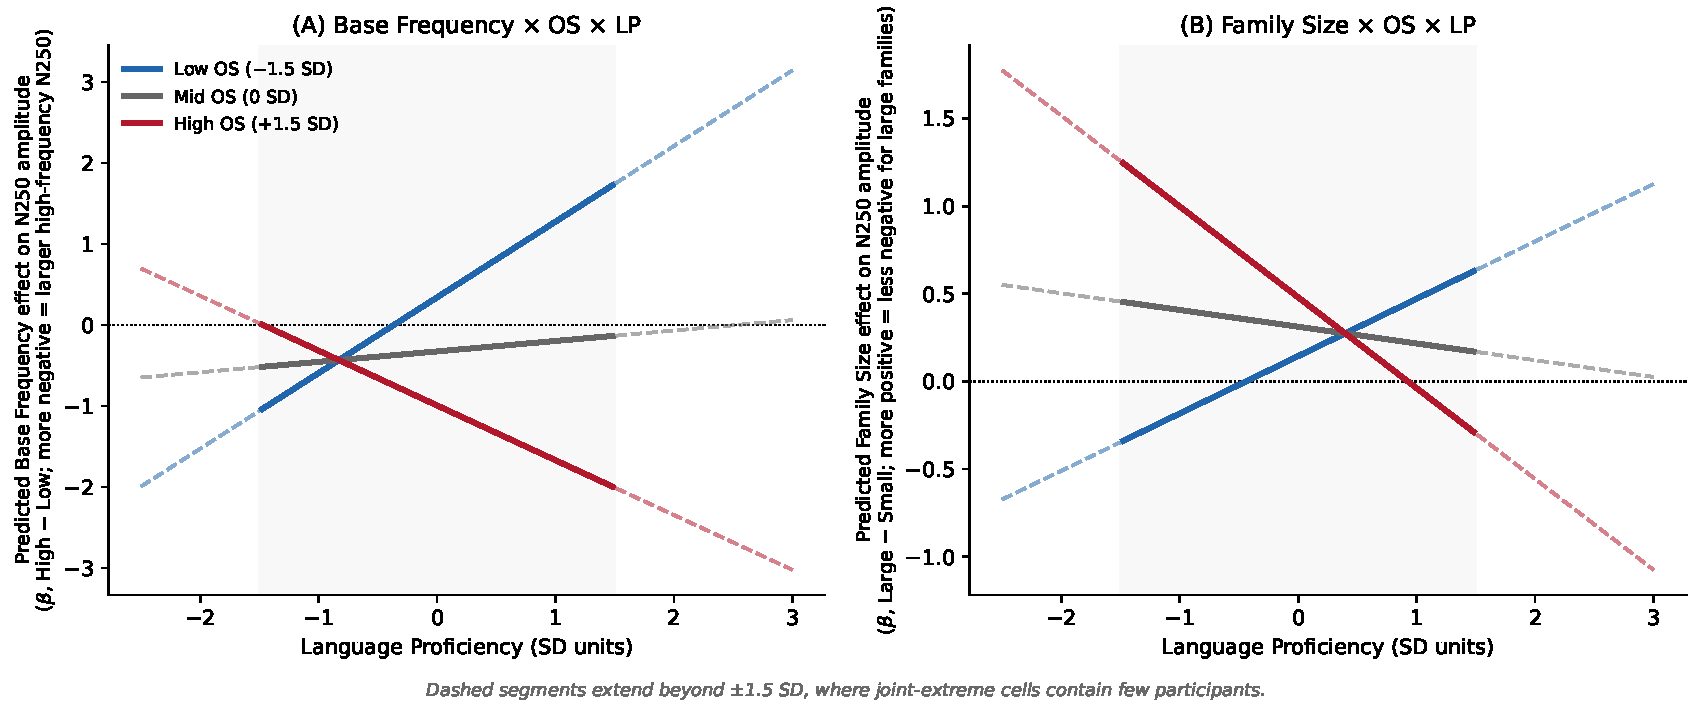
\includegraphics[width=1\textwidth]{Figure 1b Words_N250_plot}
		\caption{Predicted lexical-variable effects on N250 amplitude as a function of Language Proficiency, plotted separately for low ($-1.5$ SD), mid (0 SD), and high ($+1.5$ SD) Orthographic Sensitivity, computed from the fixed-effect estimates of each three-way model. (A) Base Frequency effect (High $-$ Low); more negative values indicate a larger high-frequency N250. (B) Family Size effect (Large $-$ Small); more positive values indicate a less negative (more positive) amplitude for large families. In both panels, solid segments span the primary reporting range ($\pm 1.5$ SD on Language Proficiency); dashed segments extend to the full observed range, where joint-extreme cells contain few participants and estimates should be treated as indicative rather than precisely estimated.}
		\label{fig:fig1b}
	\end{figure}



	\paragraph*{Words N400: Base Frequency}

	Mean N400 amplitudes for word stimuli were analysed using a linear mixed-effects model with fixed effects of Base Frequency (high vs.\ low), Language Proficiency (LP), Orthographic Sensitivity (OS), and their full three-way interaction, with the same random-effects structure as the N250 models above. The main effect of Base Frequency did not reach significance, $\beta = 0.201$, $SE = 0.106$, $t(1616) = 1.89$, $p = .060$, nor did the main effect of Language Proficiency, $\beta = 0.042$, $SE = 0.472$, $t(56) = 0.09$, $p = .929$. The main effect of Orthographic Sensitivity was significant, though only marginally so, sitting essentially at the conventional threshold, $\beta = 1.291$, $SE = 0.646$, $t(56) = 2.00$, $p = .050$, $\eta^2_p = .07$, and should be interpreted with corresponding caution.

	The three-way interaction between Base Frequency, Language Proficiency, and Orthographic Sensitivity was not significant, $\beta = -0.170$, $SE = 0.116$, $t(1616) = -1.47$, $p = .142$, consistent with a likelihood-ratio test comparing this model against a reduced model omitting the three-way term, $\chi^2(1) = 2.16$, $p = .141$. Unlike the corresponding N250 models for words, individual-difference modulation of the Base Frequency effect at the N400 did not extend to a genuine three-dimensional crossover. Of the two-way interactions, Base Frequency $\times$ Language Proficiency was significant, $\beta = 0.334$, $SE = 0.087$, $t(1616) = 3.83$, $p = .0001$, $\eta^2_p = .009$, while Base Frequency $\times$ Orthographic Sensitivity was only a non-significant trend, $\beta = 0.206$, $SE = 0.119$, $t(1616) = 1.73$, $p = .083$, and Language Proficiency $\times$ Orthographic Sensitivity was null, $\beta = -0.055$, $SE = 0.628$, $t(56) = -0.09$, $p = .931$.

	Follow-up contrasts decomposing the Base Frequency $\times$ Language Proficiency interaction, restricted to the primary reporting range of $\pm 1.5$ SD on Language Proficiency, showed that the direction of the effect shifted across this range. Near the low end of the range, the effect trended toward high-frequency words eliciting more negative N400 amplitudes than low-frequency words, though this did not reach significance (LP $= -1.5$ SD: $\beta = -0.28$, $SE = 0.17$, $t(1616) = -1.69$, $p = .090$), and was weaker still just above it (LP $= -1$ SD: $\beta = -0.12$, $SE = 0.13$, $t(1616) = -0.87$, $p = .385$). From the mean of Language Proficiency upward, the effect reversed direction and reached significance, though only marginally at the mean itself (LP $= 0$: $\beta = 0.21$, $SE = 0.11$, $t(1616) = 1.97$, $p = .049$), then strengthened clearly toward the top of the primary range (LP $= +1$ SD: $\beta = 0.54$, $SE = 0.14$, $t(1616) = 3.81$, $p < .0001$; LP $= +1.5$ SD: $\beta = 0.70$, $SE = 0.17$, $t(1616) = 4.05$, $p < .0001$). Among the small number of participants beyond this range, the same pattern continued in both directions --- the reversed-direction effect reaching significance at the lowest observed Language Proficiency scores (LP $= -2.5$ SD: $\beta = -0.61$, $p = .011$) and the expected-direction effect continuing to strengthen at the highest (LP $= +3$ SD: $\beta = 1.19$, $p < .0001$) --- but these extreme-tail estimates are based on very few participants and are reported here only as a qualitative continuation of the pattern, not as independent confirmatory tests (see Figure~\ref{fig:fig1c}, panel A).

	A corresponding breakdown across Orthographic Sensitivity, decomposing the non-significant Base Frequency $\times$ Orthographic Sensitivity trend, showed a qualitatively similar but weaker pattern within the primary range: non-significant near the low and mean end of Orthographic Sensitivity (OS $= -1.5$ SD: $\beta = -0.14$, $SE = 0.21$, $p = .518$; OS $= 0$: $\beta = 0.18$, $SE = 0.11$, $p = .083$), and reaching significance only toward the high end (OS $= +1$ SD: $\beta = 0.40$, $SE = 0.16$, $p = .011$; OS $= +1.5$ SD: $\beta = 0.51$, $SE = 0.20$, $p = .013$). Because the underlying two-way interaction did not reach significance, this breakdown is reported as a tentative, consistent pattern rather than a confirmed modulation, and should not be read as independent evidence alongside the Language Proficiency findings above. The model explained 2.7\% of variance via fixed effects ($R^2_{\mathrm{marginal}} = .027$) and 82.7\% overall ($R^2_{\mathrm{conditional}} = .827$).

	\paragraph*{Words N400: Family Size}

	A parallel model examined mean N400 amplitudes as a function of Family Size (large vs.\ small), Orthographic Sensitivity, Language Proficiency, and their full three-way interaction, with the same random-effects structure as above. The analysis revealed a significant main effect of Family Size --- words from larger morphological families elicited more positive N400 amplitudes than words from smaller families, $\beta = 0.447$, $SE = 0.064$, $t(1616) = 6.99$, $p < .0001$, $\eta^2_p = .03$. Orthographic Sensitivity also showed a significant, though again borderline, main effect, $\beta = 0.677$, $SE = 0.321$, $t(56) = 2.11$, $p = .039$, $\eta^2_p = .07$. Language Proficiency showed no reliable main effect at all, $\beta = 0.001$, $SE = 0.235$, $t(56) = 0.01$, $p = .996$.

	Unlike base frequency, none of the interaction terms in this model reached significance. The three-way interaction between Family Size, Orthographic Sensitivity, and Language Proficiency was null, $\beta = -0.037$, $SE = 0.070$, $t(1616) = -0.54$, $p = .593$, matched by a non-significant likelihood-ratio test, $\chi^2(1) = 0.29$, $p = .593$. Neither two-way interaction approached significance either --- Family Size $\times$ Orthographic Sensitivity, $\beta = 0.089$, $SE = 0.072$, $t(1616) = 1.25$, $p = .213$, or Family Size $\times$ Language Proficiency, $\beta = -0.073$, $SE = 0.052$, $t(1616) = -1.39$, $p = .164$ --- nor did Orthographic Sensitivity $\times$ Language Proficiency, $\beta < 0.001$, $SE = 0.312$, $t(56) = 0.001$, $p = .9995$. Of the four word ERP models reported here, this is the only one in which individual differences show no detectable influence, at any order, on the lexical-variable effect itself: the Family Size effect at the N400 is robust and uniform across the full range of both Orthographic Sensitivity and Language Proficiency (see Figure~\ref{fig:fig1c}, panel B). The model explained 3.1\% of variance via fixed effects ($R^2_{\mathrm{marginal}} = .031$) and 75.7\% overall ($R^2_{\mathrm{conditional}} = .757$).

	\begin{figure}[htbp]
		\centering
		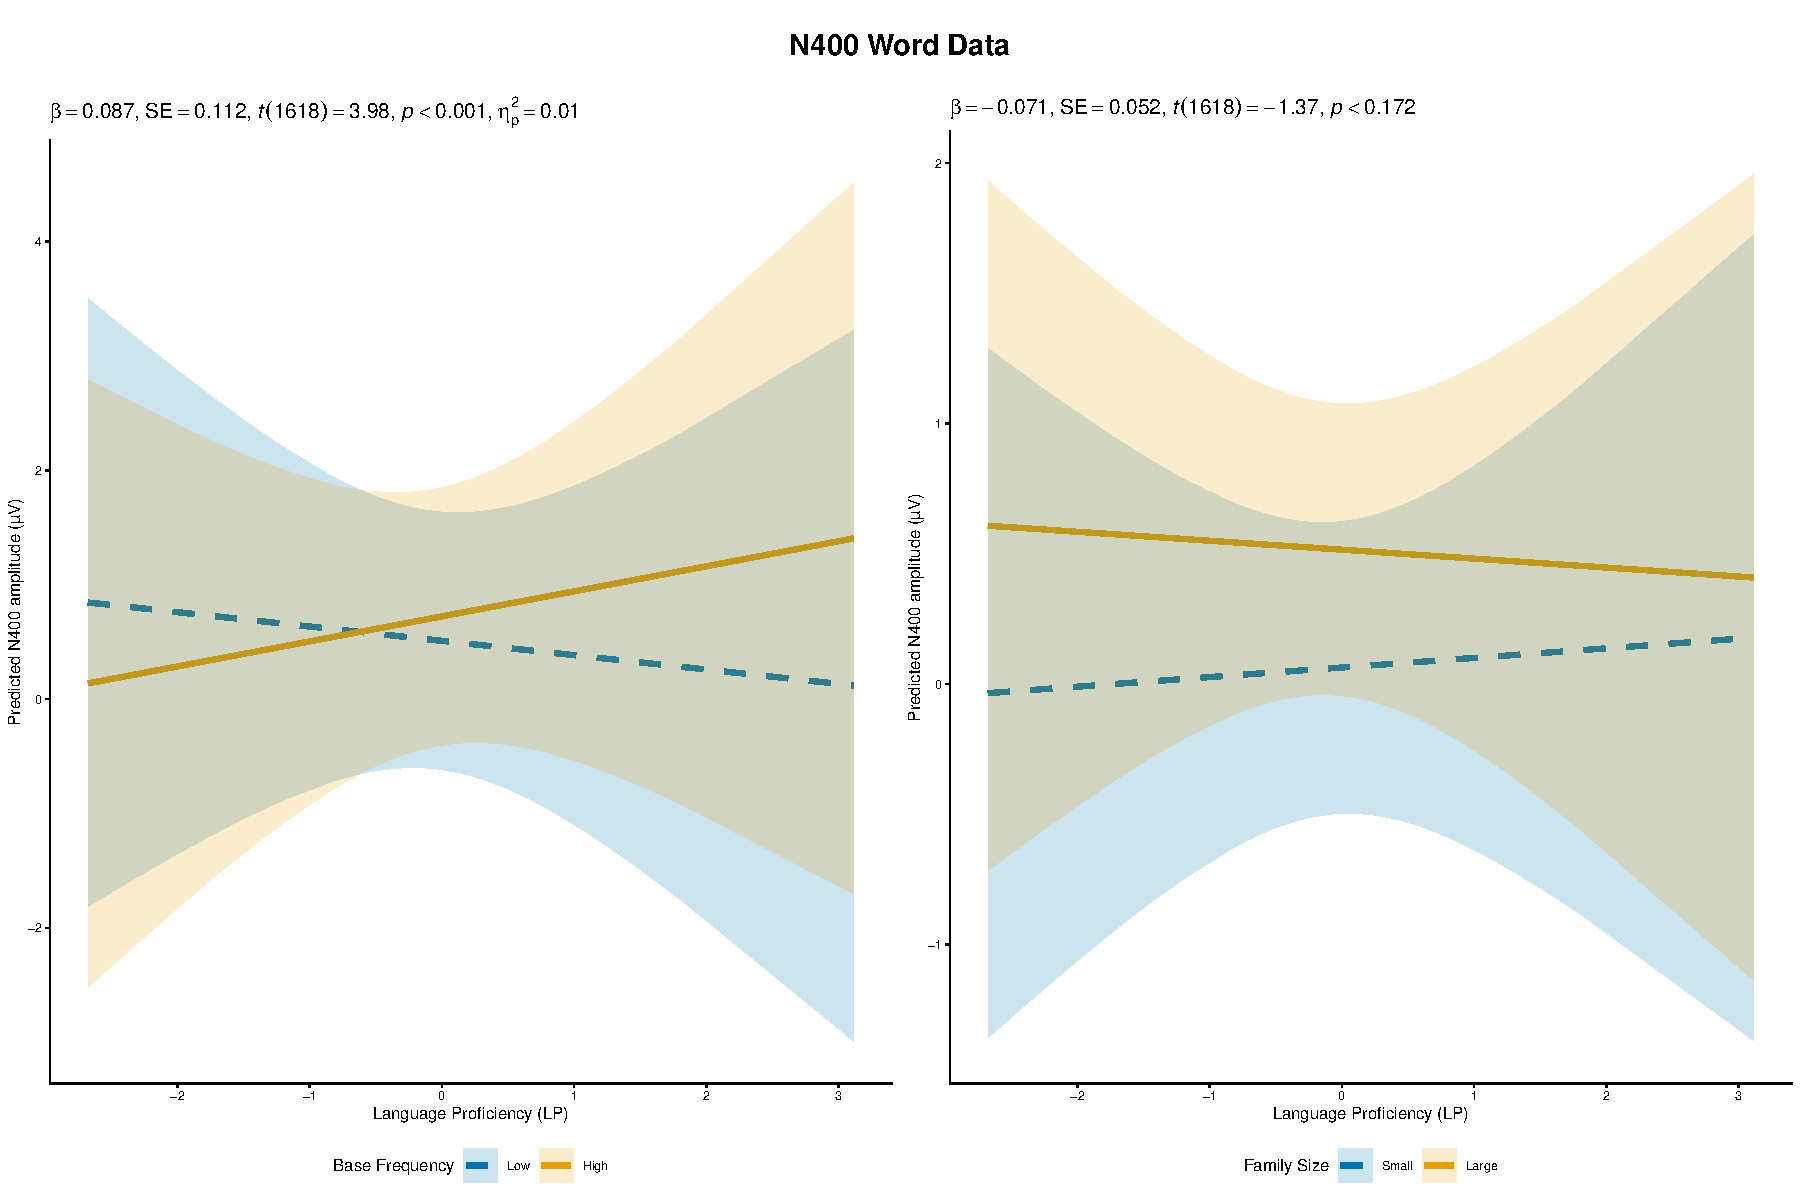
\includegraphics[width=1\textwidth]{Figure 1c Words_N400_BFxLP_plot}
		\caption{Predicted N400 amplitude as a function of Language Proficiency, plotted separately by condition, using estimated marginal means and 95\% confidence intervals in both panels. (A) Base Frequency (High vs.\ Low): the significant Base Frequency $\times$ Language Proficiency two-way interaction reverses in direction across the range, though the three-way interaction with Orthographic Sensitivity was not significant; estimates shown are from the follow-up contrasts reported in text. (B) Family Size (Large vs.\ Small): no interaction with Language Proficiency or Orthographic Sensitivity was significant, and these estimated marginal means were computed for illustration only, not as formal follow-up tests. The two lines remain approximately parallel with heavily overlapping confidence intervals throughout the observed range, visually confirming the absence of any individual-difference modulation.}
		\label{fig:fig1c}
	\end{figure}

	\subsection{Nonwords}
	
	\paragraph*{Nonwords RT}
	Reaction times (RTs) for correct lexical decisions to nonwords were analyzed using a linear mixed-effects model with fixed effects of Morphological Complexity (simple vs.\ complex), Base Frequency, Family Size, Orthographic Sensitivity (OS), and Language Proficiency (LP). The model included random intercepts for participants and items and by-participant random slopes for Complexity. The analysis revealed a strong main effect of Morphological Complexity—complex nonwords elicited slower responses than simple nonwords, $M_{\mathrm{complex}} = 718.9$ ms, 95\% CI $[695.2, 743.4]$, $M_{\mathrm{simple}} = 684.6$ ms, 95\% CI $[661.5, 708.5]$, $\beta = 0.049$, $SE = 0.005$, $t(62.68) = 9.13$, $p < .001$, $\eta^2_p = .57$. (See Figure \ref{fig:fig2a} A) In addition, Base Frequency exerted a reliable inhibitory effect, $\beta = 0.015$, $SE = 0.005$, $t(98.21) = 3.05$, $p = .003$, $\eta^2_p = .09$, such that nonwords derived from higher-frequency bases were responded to more slowly than those from lower-frequency bases. Family Size did not significantly influence response times, $\beta = -0.006$, $SE = 0.005$, $t(96.64) = -1.24$, $p = .22$. Orthographic Sensitivity showed a significant main effect, with higher-sensitivity participants responding more quickly overall, $\beta = -0.041$, $SE = 0.018$, $t(62.21) = -2.23$, $p = .030$, $\eta^2_p = .07$. In contrast, there was no effect of Language Proficiency on nonword RTs, $\beta = 0.003$, $SE = 0.012$, $t(62.91) = 0.28$, $p = .78$. The model explained 5.0\% of the variance via fixed effects ($R^2_{\mathrm{marginal}} = .050$) and 49.4\% overall ($R^2_{\mathrm{conditional}} = .494$). Taken together, these results indicate that nonword decision latencies are strongly shaped by morphological complexity and item-level lexical familiarity, particularly base frequency, while individual differences primarily affect overall response efficiency, with more orthographically sensitive readers responding more quickly across conditions. (See Figure \ref{fig:fig2a})
	
	\begin{figure}
		\centering
		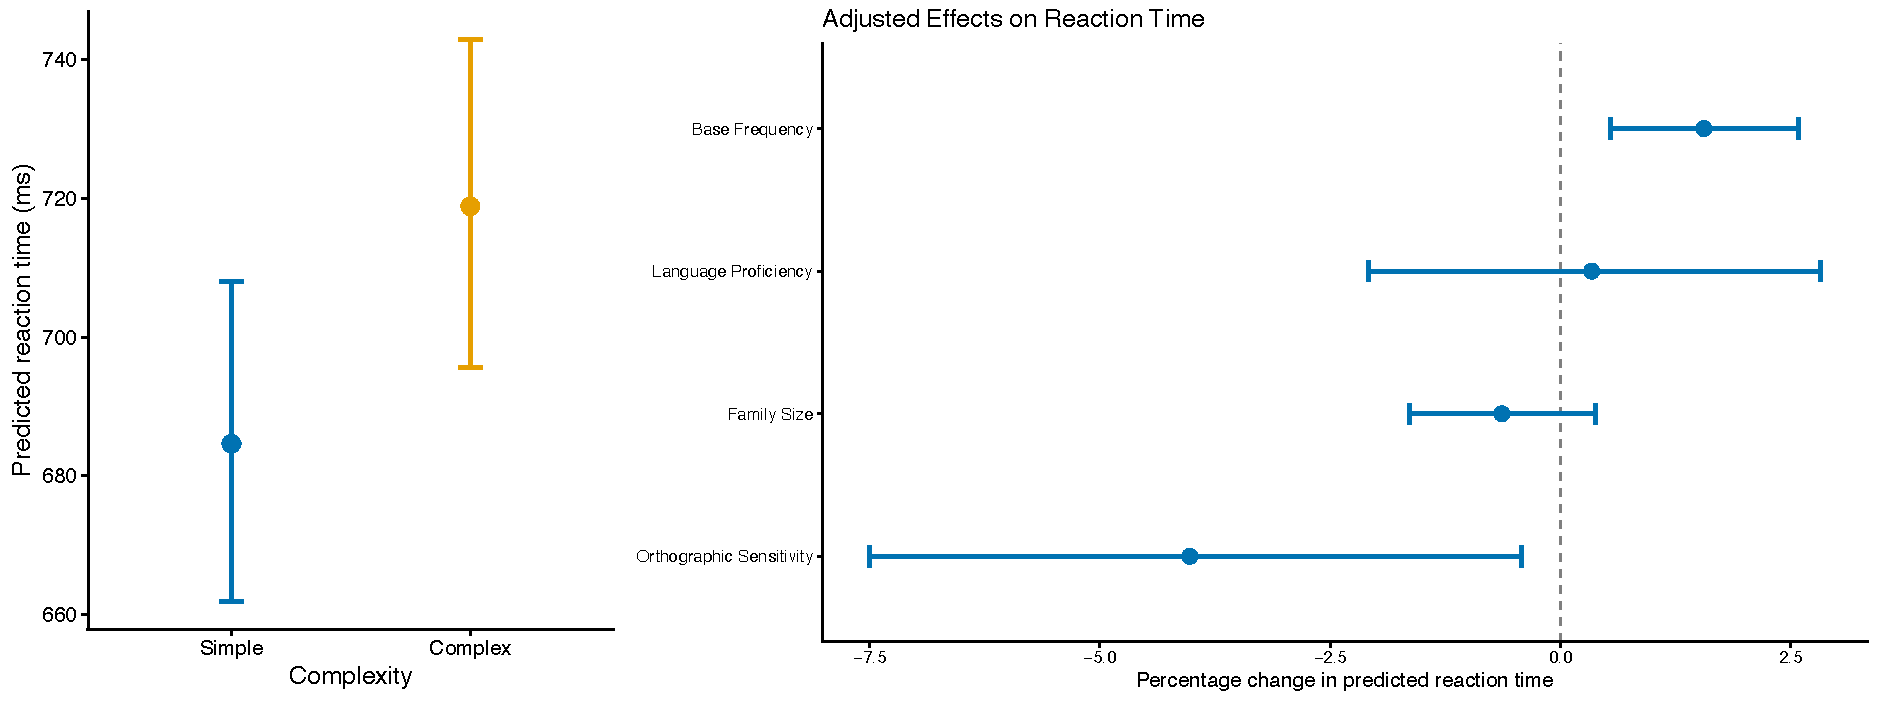
\includegraphics[width=1\textwidth]{Figure 2a NonWords_RT_coefficient_plot}
		\caption{Nonword reaction time results. (a) Predicted reaction time (ms) by complexity condition (Simple vs Complex), showing the significant complexity cost. (b) Adjusted percentage change in predicted reaction time associated with each predictor (Base Frequency, Family Size, Language Proficiency, Orthographic Sensitivity), with error bars representing confidence intervals. Complexity and Base Frequency were associated with significant increases in reaction time, and Orthographic Sensitivity with a significant decrease; Family Size and Language Proficiency were not significant predictors.}
		\label{fig:fig2a}
	\end{figure}
	
	
	\paragraph*{Nonwords N250}
	
	Mean N250 amplitudes for nonword stimuli were analysed using a linear mixed-effects model with fixed effects of Morphological Complexity, Orthographic Sensitivity (OS), Language Proficiency (LP), and Family Size, including the two-way interaction between Complexity and each individual difference dimension individually, together with the full three-way interaction among OS, LP, and Family Size, consistent with the fully-crossed model structure described in the Methods. The model included random intercepts for participants and for electrode site nested within participant.

	The analysis revealed a significant main effect of Morphological Complexity, with complex nonwords eliciting more negative N250 amplitudes than simple nonwords overall (EMM: Complex $= -0.759\,\mu$V $[-1.156, -0.363]$, Simple $= -0.526\,\mu$V $[-0.922, -0.130]$), $\beta = -0.233$, $SE = 0.050$, $t(4852) = -4.64$, $p < .0001$, $\eta^2_p = .004$. Family Size yielded a significant main effect, $\beta = 0.181$, $SE = 0.050$, $t(4852) = 3.61$, $p = .0003$, $\eta^2_p = .003$, with large-family nonwords eliciting less negative amplitudes than small-family nonwords. Neither OS nor LP yielded reliable main effects, $\beta = 0.301$, $SE = 0.218$, $t(56) = 1.38$, $p = .172$; $\beta = -0.233$, $SE = 0.159$, $t(56) = -1.46$, $p = .149$, respectively.

	The Complexity $\times$ OS interaction was significant, $\beta = 0.392$, $SE = 0.056$, $t(4852) = 6.98$, $p < .0001$, $\eta^2_p = .010$. Follow-up contrasts examined the complexity effect across the observed OS range ($-1.9$ to $+1.9$ SD). The complexity effect was large and reliable at OS $= -1.9$ SD ($\Delta = 0.990\,\mu$V, $t = 8.29$, $p < .0001$) and at OS $= -1$ SD ($\Delta = 0.642\,\mu$V, $t = 8.33$, $p < .0001$), attenuated but still significant at mean OS ($\Delta = 0.250\,\mu$V, $t = 4.98$, $p < .0001$), and reversed in direction but only marginally significant at OS $= +1$ SD ($\Delta = -0.142\,\mu$V, $t = -1.93$, $p = .053$). At the upper extreme of the observed OS range (OS $= +1.9$ SD) the reversal was significant ($\Delta = -0.490\,\mu$V, $t = -4.27$, $p < .0001$). Examination of estimated marginal means indicated that this reversal was driven primarily by the trajectory of complex nonwords, which decreased in negativity across the OS range (EMM: $-1.720\,\mu$V at OS $= -1.9$ SD to $+0.160\,\mu$V at OS $= +1.9$ SD), while simple nonwords also decreased in negativity but more slowly (EMM: $-0.720\,\mu$V at OS $= -1.9$ SD to $-0.340\,\mu$V at OS $= +1.9$ SD). (See Figure \ref{fig:fig2b} A)

	The Complexity $\times$ LP interaction was also significant, $\beta = 0.358$, $SE = 0.041$, $t(4852) = 8.76$, $p < .0001$, $\eta^2_p = .02$. Follow-up contrasts examined the complexity effect across the observed LP range ($-2.5$ to $+3.0$ SD). The complexity effect was large and reliable at LP $= -2.5$ SD ($\Delta = 1.110\,\mu$V, $t = 9.92$, $p < .0001$) and at LP $= -1$ SD ($\Delta = 0.574\,\mu$V, $t = 9.05$, $p < .0001$), attenuated but still significant at mean LP ($\Delta = 0.216\,\mu$V, $t = 4.31$, $p < .0001$), and significantly reversed at LP $= +1$ SD ($\Delta = -0.141\,\mu$V, $t = -2.14$, $p = .032$) and strongly reversed at LP $= +3$ SD ($\Delta = -0.860\,\mu$V, $t = -6.38$, $p < .0001$). In contrast to the OS pattern, examination of estimated marginal means indicated that the LP reversal was driven primarily by the trajectory of simple nonwords, which became increasingly negative across the LP range (EMM: $+0.420\,\mu$V at LP $= -2.5$ SD to $-1.700\,\mu$V at LP $= +3.0$ SD), while complex nonwords remained essentially flat (EMM: $-0.690\,\mu$V at LP $= -2.5$ SD to $-0.840\,\mu$V at LP $= +3.0$ SD). Participant LP scores ranged from $-2.67$ to $+3.11$ and OS scores ranged from $-1.98$ to $+1.93$, confirming that all contrasts are grounded in observed data rather than extrapolation. (See Figure \ref{fig:fig2b} B)
	
	\begin{figure}[htbp]
		\centering
		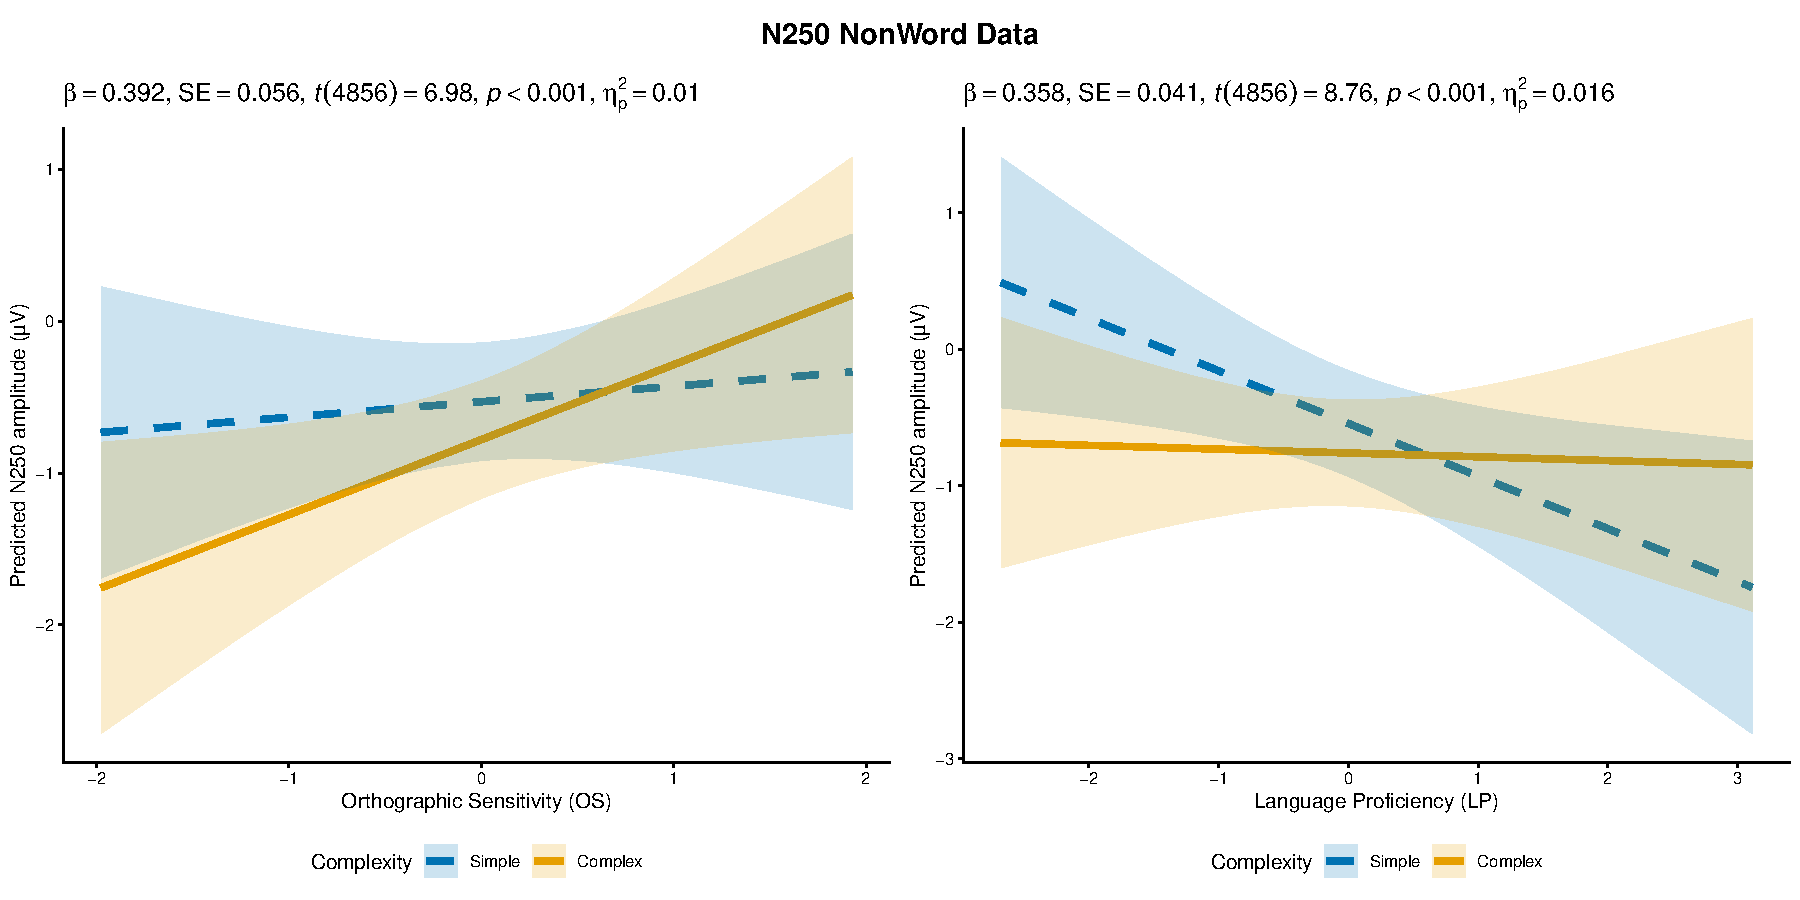
\includegraphics[width=1\textwidth]{Figure 2b NonWords_N250_plot}
		\caption{Predicted N250 amplitude for nonwords as a function of Orthographic Sensitivity (A) and Language Proficiency (B), plotted separately by Complexity (Simple vs.\ Complex), using estimated marginal means and 95\% confidence intervals from the follow-up contrasts reported in text. In both panels, the complexity cost (Complex more negative than Simple) is large at low values of the individual-difference dimension and reverses at high values, consistent with the significant Complexity $\times$ OS and Complexity $\times$ LP interactions.}
		\label{fig:fig2b}
	\end{figure}

	Beyond this established complexity-driven pattern, Family Size itself entered a significant three-way interaction with Orthographic Sensitivity and Language Proficiency, $\beta = 0.139$, $SE = 0.055$, $t(4852) = 2.54$, $p = .011$, $\eta^2_p = .001$, robust to the exclusion of the single participant with the most extreme Language Proficiency score ($\beta = 0.137$, $t = 2.49$, $p = .013$ with that participant excluded). As with the corresponding word N250 models, this interaction took the form of a crossover rather than a simple amplification --- but unlike the word-level crossovers, its statistical confirmation was asymmetric across the two poles of the primary $\pm 1.5$ SD reporting range. Decomposing by Orthographic Sensitivity, the Language Proficiency slope-difference between small- and large-family nonwords was significantly positive at low OS (OS $= -1.5$ SD: $\beta = 0.24$, $SE = 0.09$, $t(4852) = 2.72$, $p = .007$) and near zero at the mean of OS ($\beta = 0.03$, $SE = 0.04$, $t = 0.73$, $p = .465$), but only a non-significant trend at high OS within the primary range (OS $= +1.5$ SD: $\beta = -0.18$, $SE = 0.10$, $t = -1.86$, $p = .062$), reaching significance only just beyond it (OS $= +1.9$ SD: $\beta = -0.23$, $t = -2.02$, $p = .044$). The mirror-image decomposition, examining the Orthographic Sensitivity slope-difference across Language Proficiency, showed the complementary asymmetry: non-significant at low and mean LP within the primary range (LP $= -1.5$ SD: $\beta = 0.14$, $p = .148$; LP $= 0$: $\beta = -0.06$, $p = .255$) but significantly negative from LP $= +1$ SD upward ($\beta = -0.20$, $p = .009$ at LP $= +1$; $\beta = -0.27$, $p = .006$ at LP $= +1.5$), strengthening further beyond the primary range (LP $= +3$ SD: $\beta = -0.48$, $p = .005$). Together, the two decompositions describe a single underlying crossover surface whose statistical confirmation is stronger toward the low-OS/high-LP pole than the high-OS/low-LP pole within the primary reporting range (see Figure~\ref{fig:fig2b2}).

	A parallel model substituting base frequency for family size confirmed the specificity of this three-way interaction: the corresponding Orthographic Sensitivity $\times$ Language Proficiency $\times$ Base Frequency interaction was not significant, $\beta = 0.135$, $SE = 0.142$, $t(4852) = 0.95$, $p = .343$.

	The four-way interaction between Complexity, Orthographic Sensitivity, Language Proficiency, and Family Size was tested in a fully saturated model and found non-significant, $\beta = -0.084$, $SE = 0.109$, $t(4852) = -0.77$, $p = .439$, confirmed by an isolated likelihood-ratio test comparing this term against a model containing all lower-order terms, $\chi^2(1) = 0.60$, $p = .439$, justifying its exclusion from the confirmatory model reported above. Within that same saturated model, one additional term outside the confirmatory design reached significance: Complexity $\times$ Orthographic Sensitivity $\times$ Family Size, $\beta = 0.261$, $SE = 0.112$, $t(4852) = 2.33$, $p = .020$. This term was not part of the theoretically motivated model structure and is noted here for completeness rather than interpreted further.

	The model explained 3.4\% of variance via fixed effects ($R^2_{\mathrm{marginal}} = .034$) and 57.7\% overall ($R^2_{\mathrm{conditional}} = .577$).

	\begin{figure}[htbp]
		\centering
		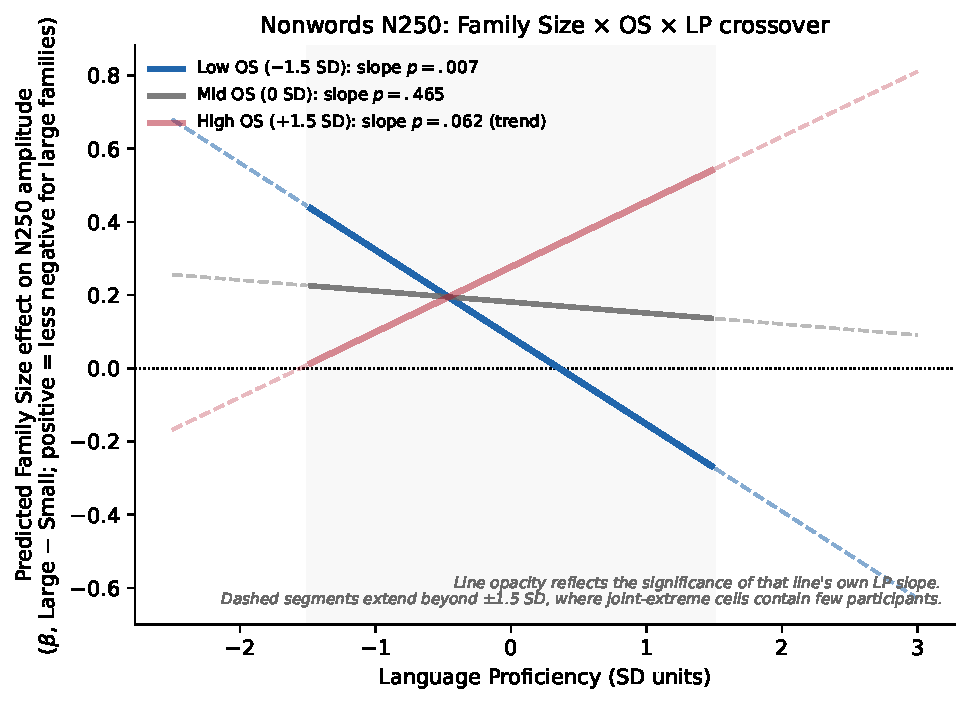
\includegraphics[width=0.65\textwidth]{Figure 2b.2 NonWords_N250_FSxOSxLP_plot}
		\caption{Predicted Family Size effect (Large $-$ Small) on nonword N250 amplitude as a function of Language Proficiency, plotted separately for low ($-1.5$ SD), mid (0 SD), and high ($+1.5$ SD) Orthographic Sensitivity, computed from the fixed-effect estimates of the Family Size $\times$ OS $\times$ LP model. Line opacity reflects the significance of that line's own Language Proficiency slope: the low-OS line (full opacity) reflects a significant slope ($p = .007$); the high-OS line (reduced opacity) reflects a non-significant trend within the primary range ($p = .062$). Solid segments span the primary reporting range ($\pm 1.5$ SD on Language Proficiency); dashed segments extend to the full observed range, where joint-extreme cells contain few participants and estimates should be treated as indicative rather than precisely estimated.}
		\label{fig:fig2b2}
	\end{figure}

	\paragraph*{Nonwords N400}
	Mean N400 amplitudes for nonword stimuli were analysed using a single symmetric linear mixed-effects model including fixed effects of Morphological Complexity, Morphological Family Size, Language Proficiency (LP), Orthographic Sensitivity (OS), and all interactions among Complexity, Family Size, and each individual difference dimension separately. The model included random intercepts for participants and for electrode site nested within participant. This symmetric structure permitted direct comparison of the roles of LP and OS in modulating the joint influence of morphological complexity and family size at the N400, providing a formal test of the predicted dissociation between the two dimensions.
	
	The analysis revealed a significant main effect of Morphological Complexity, with complex nonwords eliciting more negative N400 amplitudes than simple nonwords, $\beta = -0.469$, $SE = 0.061$, $t(4851) = -7.64$, $p < .001$, $\eta^2_p = .010$. Family Size did not yield a reliable main effect, $\beta = 0.085$, $SE = 0.061$, $t(4851) = 1.38$, $p = .168$. Neither LP, $\beta = 0.011$, $SE = 0.255$, $t(57) = 0.045$, $p = .964$, nor OS, $\beta = 0.381$, $SE = 0.350$, $t(57) = 1.09$, $p = .281$, yielded reliable main effects.
	
	The Complexity $\times$ Family Size interaction was significant, $\beta = -0.446$, $SE = 0.123$, $t(4851) = -3.63$, $p < .001$, indicating that the N400 complexity effect was larger for nonwords from large morphological families than for those from small families, averaged across both individual difference dimensions. The Complexity $\times$ LP interaction was significant, $\beta = 0.254$, $SE = 0.050$, $t(4851) = 5.08$, $p < .001$, $\eta^2_p = .005$. Follow-up contrasts examined the complexity effect across the observed LP range ($-2.5$ to $+3.0$ SD), averaged over family size. The complexity effect was large and reliable at LP $= -2.5$ SD ($\Delta = 1.090\,\mu$V, $t = 7.99$, $p < .001$) and at LP $= -1$ SD ($\Delta = 0.710\,\mu$V, $t = 9.19$, $p < .001$), attenuated at mean LP ($\Delta = 0.460\,\mu$V, $t = 7.48$, $p < .001$), and further reduced but still significant at LP $= +1$ SD ($\Delta = 0.210\,\mu$V, $t = 2.54$, $p = .011$). At the upper limit of the observed LP range (LP $= +3$ SD) the complexity effect reversed in direction but did not reach significance ($\Delta = -0.300\,\mu$V, $t = -1.84$, $p = .065$).  The Family Size $\times$ LP interaction was also significant, $\beta = 0.122$, $SE = 0.050$, $t(4851) = 2.45$, $p = .015$, indicating that the influence of family size on N400 amplitude varied as a function of LP; this interaction is qualified by the three-way interaction reported below. The Complexity $\times$ OS interaction was significant, $\beta = 0.240$, $SE = 0.069$, $t(4851) = 3.49$, $p < .001$, $\eta^2_p = .003$, indicating that the complexity effect also attenuated with increasing OS, though as reported below, OS did not selectively modulate the joint influence of complexity and family size. The Family Size $\times$ OS interaction was not significant, $\beta = 0.066$, $SE = 0.069$, $t(4851) = 0.955$, $p = .340$.
	
	Critically, the three-way Complexity $\times$ Family Size $\times$ LP interaction was significant, $\beta = 0.229$, $SE = 0.100$, $t(4851) = 2.29$, $p = .022$, $\eta^2_p = .001$, while the corresponding Complexity $\times$ Family Size $\times$ OS interaction was not significant, $\beta = 0.143$, $SE = 0.138$, $t(4851) = 1.04$, $p = .300$. This asymmetry --- LP driving the three-way interaction while OS does not --- constitutes the primary evidence for the predicted dissociation between the two individual difference dimensions at the N400.
	
	Follow-up interaction contrasts for the significant LP three-way examined the Complexity $\times$ Family Size interaction separately across the observed LP range ($-2.5$ to $+3.0$ SD). At LP $= -2.5$ SD, the Complexity $\times$ Family Size interaction was large and highly reliable ($\Delta = -1.010\,\mu$V, $t = -3.70$, $p < .001$) --- the complexity effect was substantially larger for large-family nonwords ($\Delta = 1.600\,\mu$V, $t = 8.26$, $p < .001$) than for small-family nonwords ($\Delta = 0.590\,\mu$V, $t = 3.03$, $p = .002$), reflecting disproportionately strong semantic processing demands when both morphological complexity and family richness are high. At LP $= -1$ SD the interaction remained large and significant ($\Delta = -0.670\,\mu$V, $t = -4.31$, $p < .001$), with complexity effects again larger for large-family ($\Delta = 1.050\,\mu$V, $t = 9.55$, $p < .001$) than small-family nonwords ($\Delta = 0.380\,\mu$V, $t = 3.45$, $p = .001$). At mean LP the interaction remained significant but attenuated ($\Delta = -0.440\,\mu$V, $t = -3.58$, $p < .001$), with complexity effects larger for large-family ($\Delta = 0.680\,\mu$V, $t = 7.82$, $p < .001$) than small-family nonwords ($\Delta = 0.240\,\mu$V, $t = 2.76$, $p = .006$). At LP $= +1$ SD the interaction was no longer significant ($\Delta = -0.210\,\mu$V, $t = -1.31$, $p = .192$), and at LP $= +3$ SD --- the upper limit of the observed LP range --- the interaction reversed in sign but did not reach significance ($\Delta = 0.250\,\mu$V, $t = 0.76$, $p = .450$).
	
	To characterise the nature of the LP modulation more precisely, follow-up contrasts examined the family size effect within complex nonwords specifically across the observed LP range. At LP $= -2.5$ SD, large-family complex nonwords elicited substantially more negative N400 amplitudes than small-family complex nonwords ($\Delta = 0.720\,\mu$V, $t = 3.74$, $p < .001$). This difference decreased monotonically with increasing LP: at LP $= -1$ SD ($\Delta = 0.370\,\mu$V, $t = 3.36$, $p = .001$), at mean LP ($\Delta = 0.130\,\mu$V, $t = 1.53$, $p = .127$), and at LP $= +1$ SD the difference was negligible and non-significant ($\Delta = -0.100\,\mu$V, $t = -0.91$, $p = .360$). At LP $= +3$ SD the pattern reversed significantly --- small-family complex nonwords now elicited more negative N400 amplitudes than large-family complex nonwords ($\Delta = -0.580\,\mu$V, $t = -2.49$, $p = .013$) --- indicating that for highly proficient readers, morphological family richness facilitates rather than amplifies semantic integration demands for complex nonwords.  (See Figure \ref{fig:fig2c1})
	
	\begin{figure}
		\centering
		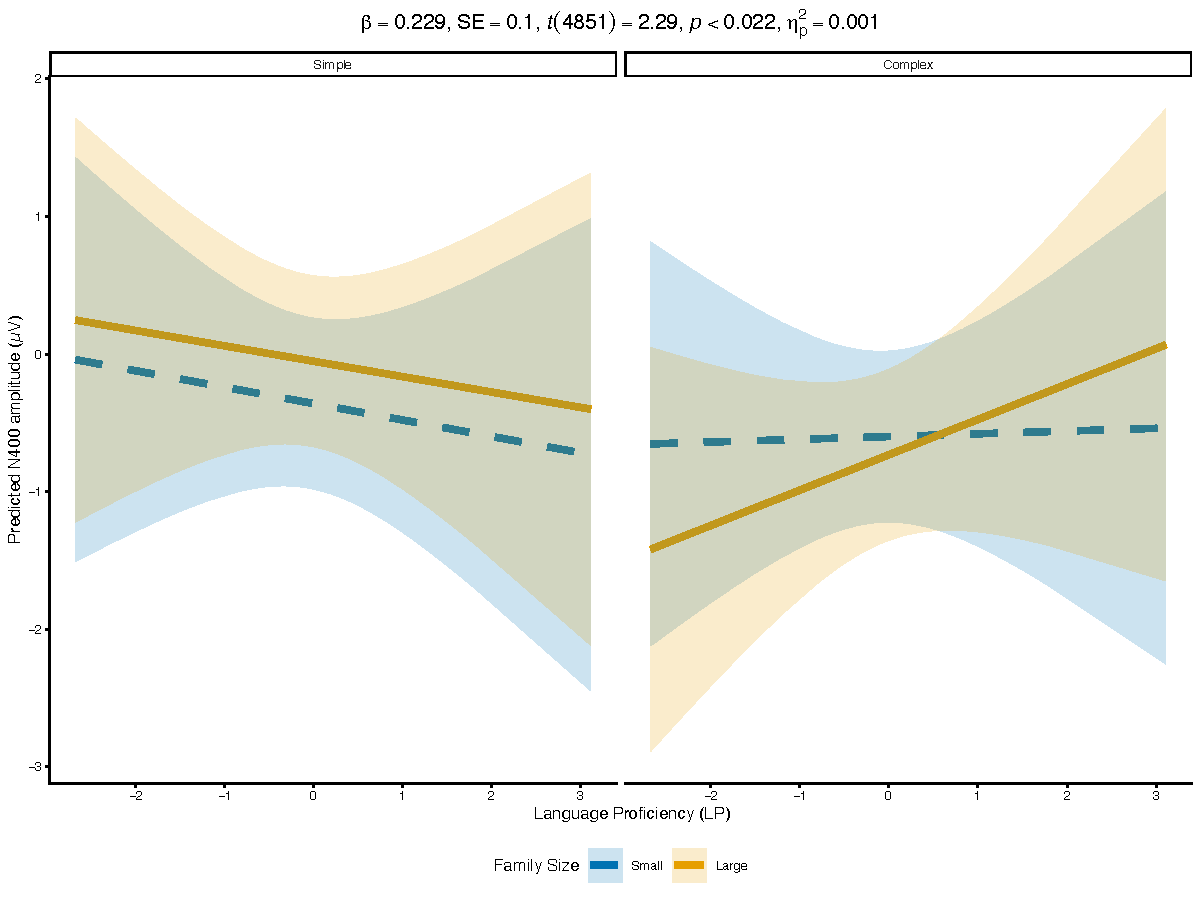
\includegraphics[width=0.75\textwidth]{Figure 2c.1 NonWords_N400_LP_plot}
		\caption{Predicted N400 amplitude for nonwords as a function of Language Proficiency (LP), plotted separately by family size (Small vs Large) within each complexity condition (Simple, Complex), illustrating the Complexity × Family Size × LP three-way interaction. Within simple nonwords, the family size effect is small and relatively stable across the LP range. Within complex nonwords, the pattern shifts systematically with LP: large-family nonwords elicit substantially more negative amplitudes than small-family nonwords at low LP, this difference diminishes through the mid-range of LP, and at the upper end of the observed range the pattern reverses, with small-family nonwords eliciting more negative amplitudes than large-family nonwords. Shaded ribbons represent 95\% confidence intervals.
		}
		\label{fig:fig2c1}
	\end{figure}
	
	
	
	Although the Complexity $\times$ Family Size $\times$ OS interaction was not significant,  $\beta = 0.143$, $SE = 0.138$, $t(4851) = 1.04$, $p = .30$, descriptive contrasts were conducted across the observed OS range ($-1.9$ to $+1.9$ SD) to characterise the nature of this null result and to directly compare the OS pattern with the LP pattern reported above. The Complexity $\times$ Family Size interaction was significant at low OS (OS $= -1.9$ SD: $\Delta = -0.730\,\mu$V, $t = -2.48$, $p = .013$; OS $= -1$ SD: $\Delta = -0.600\,\mu$V, $t = -3.18$, $p = .001$) and at mean OS ($\Delta = -0.460\,\mu$V, $t = -3.72$, $p < .001$), reflecting a pattern qualitatively similar to that seen at low LP. However, unlike the LP pattern, the interaction attenuated monotonically without reversing as OS increased: at OS $= +1$ SD the interaction was marginal ($\Delta = -0.310\,\mu$V, $t = -1.75$, $p = .081$), and at the upper extreme of the observed OS range (OS $= +1.9$ SD) it was absent ($\Delta = -0.190\,\mu$V, $t = -0.66$, $p = .512$). Crucially, the family size effect within complex nonwords showed no significant reversal at any level of OS --- at OS $= +1.9$ SD the contrast was negligible and non-significant ($\Delta = -0.110\,\mu$V, $t = -0.55$, $p = .581$). This pattern of attenuation without reversal for OS, in contrast to the significant reversal at high LP, constitutes the clearest expression of the dissociation between the two dimensions at the N400. Participant LP scores ranged from $-2.67$ to $+3.11$ and OS scores ranged from $-1.98$ to $+1.93$, confirming that all contrasts are grounded in observed data rather than extrapolation. Model fit indices were $R^2_{\text{marginal}} = .013$ and $R^2_{\text{conditional}} = .667$. (See Figure~\ref{fig:fig2c2})
	
	\begin{figure}
		\centering
		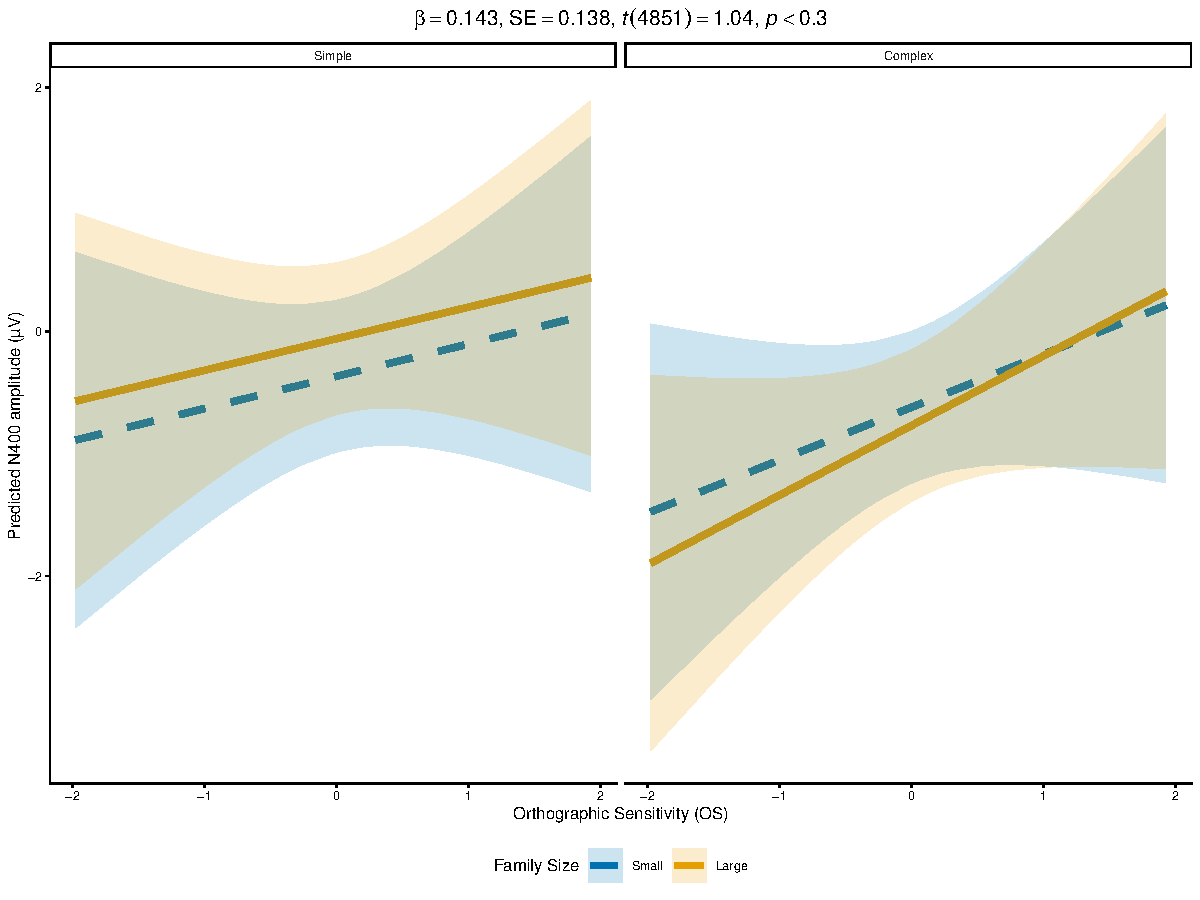
\includegraphics[width=0.75\textwidth]{Figure 2c.2 NonWords_N400_OS_plot}
		\caption{Predicted N400 amplitude for nonwords as a function of Orthographic Sensitivity (OS), plotted separately by family size (Small vs Large) within each complexity condition (Simple, Complex). Unlike the corresponding LP three-way interaction (Figure 2c), the Complexity × Family Size × OS interaction was not significant, indicating that OS does not selectively modulate the joint influence of morphological complexity and family size at the N400. This null result supports the specificity of the LP effect and constitutes part of the evidence for the predicted dissociation between the two individual difference dimensions. Shaded ribbons represent 95\% confidence intervals.}
		\label{fig:fig2c2}
	\end{figure}
	
	\section{Discussion}
	
	This study examined whether individual differences in Orthographic Sensitivity (OS) and Language Proficiency (LP) differentially modulate morphological processing at distinct temporal stages, as indexed by the N250 and N400 components of the ERP. Three findings structure the discussion that follows. First, individual differences were largely absent from behavioural response times, with the exception of an OS advantage for nonword lexical decisions, indicating that the two dimensions differ in their contribution to general lexical decision efficiency, but that neither dimension selectively influenced morphological effects in reaction times. Second, at the N250, both OS and LP modulated the complexity effect for nonword stimuli through distinct mechanisms that are developed in detail below, and OS primarily modulated the base frequency effect for word stimuli, with a smaller LP effect also present, running in the opposite direction, providing partial support for the predicted role of orthographic skill in early morpho-orthographic parsing. Third, at the N400, a model testing both OS and LP within the same analysis revealed that LP selectively drove the three-way interaction between morphological complexity and family size for nonword stimuli, while the corresponding OS interaction was not significant, constituting the clearest evidence for the predicted dissociation between the two dimensions. LP also shaped base frequency effects for word stimuli: the facilitatory effect of high base frequency, a more positive N400 relative to low frequency, was absent for readers low in LP but grew larger as LP increased, consistent with LP determining how form-level frequency information is weighted during semantic integration. Together these findings support a partial dissociation between OS and LP in morphological processing, with a mechanistically rich picture at the N250 and the clearest dissociation emerging at the N400.
	
	\subsection{Early Morpho-orthographic Processing: The N250}
	
	\subsubsection{Word Stimuli}
	
	For word stimuli, base frequency modulated the N250 as a function of Orthographic Sensitivity: high base frequency words elicited more negative amplitudes than low base frequency words, and this difference increased with OS, a pattern consistent with the prediction that early form-based processing is selectively shaped by the precision of sublexical orthographic representations. Morphological family size also modulated the N250 as a main effect, with large-family words eliciting less negative amplitudes than small-family words. A Family Size $\times$ OS interaction showed the same qualitative trend as base frequency, though it fell short of significance ($p = .089$), suggesting that OS may extend to family size sensitivity as well, but this possibility remains tentative pending further evidence.
	
	The opposite directions of the base frequency and family size effects at the N250 are theoretically informative and can be accounted for by a distinction between form-level entrenchment and semantic reinforcement of morphological structure. Base frequency reflects how often an orthographic form has been encountered as the same lexical entry, across inflectional variants that share a stable meaning but do not create new form-meaning pairings at the lexical level. Family size, by contrast, reflects how many distinct derived words embed the base, each constituting a separate lexical entry that pairs the base form with a related but distinct meaning. Repeated encounter of the same form across multiple such meaning-bearing contexts is argued to build richer, more precise semantic representations \citep{bolgerContextVariationDefinitions2008, liLearningNovelComplex2026} as the semantic core of the base becomes more robustly specified as it is reinforced across independent form-meaning pairings. Under this account, it is the quality of the lexical representation associated with large family size, that is, the precision and richness of the semantic core built through accumulated contextual variation, that enables stronger top-down semantic feedback to the form level, facilitating orthographic identification and reducing N250 amplitude. Base frequency does not carry this semantic reinforcement; repeated encounters with a high-frequency base accumulate orthographic familiarity without necessarily building new form-meaning pairings, and its effect at the N250 therefore reflects engagement of morpho-orthographic parsing that is not necessarily supplemented by feedback from a richly specified semantic representation.
	
	The modulation of this base frequency effect by OS is consistent with the theoretical profile of this dimension. OS indexes sensitivity to sublexical orthographic structure, and readers higher in OS are more sensitive to the statistical and structural properties of sub-word units, including stem forms. For these readers, a high-frequency base strongly recruits morpho-orthographic parsing activity, producing greater N250 amplitude. The absence of a corresponding modulation by LP is consistent with the prediction that early form-based processing is specifically tied to orthographic skill rather than lexical-semantic knowledge, and supports the theoretical distinction between the two individual difference dimensions at this processing stage. As discussed below, however, the nonword data reveal a more complex picture at the N250, with LP also modulating early morphological parsing through a mechanistically distinct route.

	
	\subsubsection{Nonword Stimuli}
	
	For nonword stimuli, both OS and LP modulated the N250 complexity effect, though via independent routes rather than a single shared mechanism operating at different strengths. This constitutes a partial qualification of the predicted OS-specific modulation at the N250, but the nature of the qualification is itself theoretically informative.
	
	For readers lower in OS, complex nonwords elicited substantially more negative N250 amplitudes than simple nonwords, reflecting a large early processing cost associated with the presence of a real suffix. As OS increased, this complexity cost attenuated monotonically, reversing significantly at the upper extreme of the observed OS range (OS $= +1.9$ SD: $\Delta = -0.490\,\mu$V, $t = -4.27$, $p < .001$), though not at OS $= +1$ SD ($\Delta = -0.142\,\mu$V, $t = -1.93$, $p = .053$). Examination of estimated marginal means indicated that this reversal was driven primarily by the trajectory of complex nonwords, which decreased in negativity across the OS range (EMM: $-1.720\,\mu$V at OS $= -1.9$ SD to $+0.160\,\mu$V at OS $= +1.9$ SD), while simple nonwords also decreased in negativity but more slowly (EMM: $-0.720\,\mu$V at OS $= -1.9$ SD to $-0.340\,\mu$V at OS $= +1.9$ SD). We propose that this pattern reflects affix-led parsing \citep{taft_lexical_1975, rastleMorphologicalDecompositionBased2008}, in which the presence of a real suffix triggers morpho-orthographic parsing activity across all readers, but the efficiency with which that parsing proceeds varies with OS. On this account, for readers lower in OS, the parse is triggered by the real suffix but does not proceed efficiently, producing a processing cost for complex nonwords relative to simple ones; as OS increases, parsing becomes more efficient, reducing and eventually reversing the complexity cost. At very high OS, on this view, the parse is efficient enough that complex nonwords become easier to process than simple ones, which lack a real suffix and so do not benefit from affix-based parsing in the same way. If this account is correct, the reversal reflects the complex nonword trajectory outpacing the simple nonword trajectory as OS increases, rather than a rising processing cost for simple nonwords.
	
	The LP pattern showed a different statistical signature, and the contrast with the OS pattern points to two distinct sources of the reversal within the nonword N250 data. As with OS, the complexity effect reversed at high LP --- significantly so at LP $= +1$ SD ($\Delta = -0.141\,\mu$V, $t = -2.14$, $p = .032$) and more strongly at LP $= +3$ SD ($\Delta = -0.860\,\mu$V, $t = -6.38$, $p < .001$). However, examination of estimated marginal means indicated that a different trajectory underlies this reversal than the one underlying the OS reversal. Complex nonwords changed little across the LP range (EMM: $-0.690\,\mu$V at LP $= -2.5$ SD to $-0.820\,\mu$V at LP $= +3.0$ SD), suggesting that LP had minimal effect on the processing of complex nonwords. Instead, the reversal was driven primarily by simple nonwords becoming increasingly negative as LP increased, from $+0.420\,\mu$V at LP $= -2.5$ SD to $-1.700\,\mu$V at LP $= +3.0$ SD. We propose that this pattern reflects stem-led parsing: readers higher in LP have richer and more precise representations of stems as free morphemes with discrete lexical entries, and recognition of the stem in a nonword triggers an attempt to assign morphological structure to the whole string regardless of what follows. This proposal is consistent with \citet{beyersmannEmbeddedStemPriming2016}, who found that high proficiency readers showed embedded stem priming effects independent of whether the stem was followed by a real affix or a non-affixal ending, a pattern suggesting that stem activation in skilled readers is not contingent on affix recognition, in contrast to the standard affix-stripping account \citep{taft_lexical_1975, rastleMorphologicalDecompositionBased2008}. On this account, for complex nonwords the stem-led parse succeeds---a real stem is followed by a real suffix, yielding a valid morphological analysis---and successful parsing produces neither a cost nor a benefit at the N250, keeping amplitude stable across LP levels. For simple nonwords, on this account, the parse fails---the pseudoaffix cannot be integrated into a valid morphological structure---and this failed parse produces a processing cost that grows with LP, driving the simple nonword trajectory increasingly negative.
	
	The contrast between the two reversal patterns is informative. The OS reversal appears to be driven by the complex nonword trajectory: the real suffix triggers morpho-orthographic parsing in all readers, but higher OS readers resolve that parse more efficiently, driving complex nonwords to decrease in negativity faster than simple nonwords and eventually producing a reversal; simple nonwords would not be expected to show this pattern, since they do not contain a real suffix for affix-based parsing efficiency to act on. The LP reversal, by contrast, appears to be driven by the simple nonword trajectory: stem recognition may trigger an attempt to assign morphological structure to the whole string in higher LP readers, an attempt that succeeds for complex nonwords, keeping their amplitude stable across LP levels, but fails for simple nonwords, producing a processing cost that grows with LP. This pattern is broadly consistent with the theoretical profiles of the two dimensions: OS indexes the efficiency of sublexical orthographic processing, and its effect on early parsing is expressed specifically in the complex nonword condition, where the presence of a real affix drives differential parsing efficiency across OS levels; LP indexes the depth and precision of lexical-semantic knowledge, which we suggest may extend to knowledge of stems as free morphemes with discrete lexical entries, such that its effect on early parsing is expressed specifically in the simple nonword condition, where stem recognition triggers a parse that does not succeed, producing a cost that grows with LP. The concurrent modulation of the N250 complexity effect by both OS and LP is consistent with \citet{beyersmannEmbeddedStemPriming2016}'s suggestion that affix-chunking and embedded stem activation mechanisms may operate concurrently during early morphological segmentation, with the present data extending this proposal by suggesting that these two mechanisms are dissociable across individual difference dimensions: OS appears to index the efficiency of affix-based parsing, while LP appears to index the propensity for stem-based parsing independent of affix status.
	
	This mechanistic distinction between OS and LP at the N250 for nonwords is further grounded by the word data reported above. For familiar words, OS modulated the base frequency effect at the N250 --- a finding that reflects OS operating at the level of stem-form entrenchment in stored lexical representations. The specificity of the affix-led account for nonwords therefore does not imply that OS is exclusively sensitive to affixes in all contexts; rather, it suggests that when readers encounter a novel form for which no stored whole-word representation is available, OS-driven parsing activity is channelled specifically through affix recognition, because it is the affix that provides the primary morphological signal in that context. LP, by contrast, operates through stem recognition in both familiar and novel form processing, consistent with its profile as an index of the depth and precision of lexical-semantic representations in which stems are the primary meaning-bearing units.
	
	\subsection{Semantic Integration and the N400}
	
	The N400 findings provide the clearest support for the predicted dissociation between Orthographic Sensitivity and Language Proficiency. LP selectively modulated N400 amplitude in interaction with morphological variables across both word and nonword stimuli, consistent with the theoretical prediction that depth of lexical-semantic knowledge determines how morphological information is used during meaning access. OS modulated the overall N400 complexity effect for nonwords, reflecting a general reduction in semantic processing demands as orthographic processing becomes more efficient, but did not modulate the joint influence of morphological complexity and family size on N400 amplitude. To understand why the three-way Complexity $\times$ Family Size $\times$ LP interaction --- and not the corresponding OS interaction --- constitutes the primary test of the predicted dissociation at the N400, it is necessary to be clear about what family size indexes and why LP is predicted to modulate its influence specifically at this later processing stage. When a reader encounters a morphologically complex form, the stem may activate semantic information associated with other words in its morphological family --- derived words that share the stem and preserve its core meaning. The N400 reflects how easily that semantic activation is accessed and integrated. LP, as an index of the depth and precision of lexical-semantic representations, is predicted to determine whether the semantic richness of the morphological neighbourhood facilitates or burdens that integration process. OS, as an index of sublexical orthographic processing efficiency, is not predicted to selectively modulate this semantic process, and the data are consistent with that prediction. The asymmetry between LP and OS at the N400, established within a single model testing both dimensions simultaneously, provides the formal basis for the dissociation claim developed in the sections that follow.
	
	\subsubsection{Word Stimuli}
	
	For word stimuli, the direction of the base frequency effect at the N400 depended on LP: readers lower in LP showed greater N400 negativity for high than low frequency bases, while readers higher in LP showed the opposite pattern, with high frequency bases associated with less negative N400 amplitudes than low frequency bases. This pattern was not significant at LP $= -1$ SD but was significant at the lower and upper ends of the tested LP range, with the effect of base frequency in opposite directions at LP $= -2$ SD and LP $= +2$ SD.
	
	This finding is consistent with the Lexical Quality Hypothesis \citep{perfettiReadingAbilityLexical2007}, under which more proficient readers have more precise and fully specified lexical representations --- involving tighter connections among orthographic, phonological, and semantic information --- while less proficient readers have less precise representations in which these connections are less fully specified. Under this account, LP modulates how base frequency contributes to N400 amplitude during semantic access: for readers lower in LP, higher base frequency is associated with greater N400 negativity, suggesting that base frequency influences how actively meaning retrieval is pursued; for readers higher in LP, higher base frequency is associated with less N400 negativity, suggesting that a more familiar orthographic form supports easier meaning retrieval. The direction of the base frequency effect therefore shifts across the LP continuum, with the pattern at low LP and the pattern at high LP reflecting different expressions of how form-level familiarity interacts with the precision of lexical representations during semantic access.
	
	We note that the present data do not allow us to determine precisely why the direction of the base frequency effect shifts across LP levels. One possibility is that low and high LP readers differ in the degree to which they attempt meaning retrieval for words of varying familiarity --- low LP readers mounting a more active retrieval attempt for familiar high frequency forms and a less thorough one for less familiar low frequency forms, while high LP readers retrieve meaning efficiently regardless of base frequency but do so more easily for more familiar forms. Another possibility is that the shift reflects a single continuous process in which LP modulates the weight given to base frequency during semantic access, with the direction of the effect changing as a mathematical consequence of that modulation across the LP range. The linear interaction term in the model is consistent with both accounts and cannot distinguish between them. Accuracy data would help to adjudicate: if low LP readers are less likely to correctly recognise low frequency words --- treating them as nonwords more often --- that would support the first account; if accuracy is comparable across base frequency levels for both LP groups, the second account would be more plausible.
	
	
	\subsubsection{Nonword Stimuli}
	
	The three-way Complexity $\times$ Family Size $\times$ LP interaction illustrates the mechanistic dissociation between OS and LP at the N400, and is most readily understood by first considering why morphological family size might influence N400 amplitude at all. When a reader encounters a complex nonword like \textit{gasful}, the stem \textit{gas} activates other words in its morphological family --- \textit{gases}, \textit{gassy}, \textit{gaseous} --- each of which shares the stem's core meaning. A stem with a large morphological family activates more semantic associates than one with a small family, creating a richer semantic network that must be evaluated against a form that has no stored lexical entry. Whether this richer activation constitutes a processing burden or a processing advantage depends on two factors simultaneously, as the three-way interaction reveals: whether the form signals a valid morphological structure --- which determines whether the stem's morphological family is recruited during processing --- and the precision of the reader's lexical-semantic representations, indexed by LP. For simple nonwords, the pseudoaffix does not signal a valid morphological structure. Without that morphological signal, the reader does not parse the string as a derived form and does not recruit the stem's morphological family as part of semantic processing. If family-level semantic activation is not recruited, its richness cannot influence processing, and LP --- which determines how efficiently that activation is leveraged --- has nothing to modulate. This is why the family size effect for simple nonwords is small and does not vary with LP. For complex nonwords, by contrast, the real suffix signals valid morphological structure, triggering recruitment of the stem's morphological family and making LP the critical determinant of whether that activation facilitates or burdens processing.
	
	Figure~\ref{fig:fig2c1} illustrates how LP modulates the family size effect specifically for complex nonwords. The figure plots N400 amplitude as a function of LP separately for large and small family nonwords, with simple and complex nonwords shown in separate panels. For simple nonwords, the family size lines are relatively flat and parallel across the LP range, consistent with the account above. For complex nonwords, the picture is strikingly different: as LP increases, the amplitude for large-family complex nonwords decreases substantially, while the amplitude for small-family complex nonwords remains relatively stable. At low LP, large-family complex nonwords elicit considerably more negative N400 amplitudes than small-family complex nonwords; at high LP, this difference reverses, with large-family complex nonwords eliciting less negative amplitudes than small-family ones. It is this divergence of the large-family and small-family trajectories specifically within complex nonwords, and the stability of those trajectories within simple nonwords, that constitutes the three-way interaction.
	
	This pattern is interpretable within the Lexical Quality Hypothesis \citep{perfettiReadingAbilityLexical2007}, under which more proficient readers have more precise and fully specified lexical representations, involving tighter connections among orthographic, phonological, and semantic information. Under this framework, what differs across LP levels is not the quantity of semantic activation generated by a large morphological family, but the quality of the representations that are activated. High LP readers have precise, well-specified representations of the stem's morphological relatives --- each family member is a distinct, fully specified lexical entry with a clear form-meaning relationship. When such a reader encounters a large-family complex nonword, the activated semantic network is organised and coherent, and the reader can draw on this organised knowledge to efficiently evaluate the novel form: they recognise the morphological structure, identify the stem and its semantic core, and process the novel derived form against a well-specified representational background. The result is less negative N400 amplitude for large-family complex nonwords at high LP --- the richness of the family facilitates rather than burdens processing. For readers lower in LP, the same network is activated but the representations of family members are less precise and less fully specified. The reader cannot draw on this activation as efficiently, and the additional semantic content generated by a large family creates processing demands that are difficult to resolve against a novel form with no lexical entry. The result is more negative N400 amplitude for large-family complex nonwords at low LP --- the richness of the family amplifies rather than reduces processing demands.
	
	This account is also consistent with the distinction between base frequency and family size developed in the context of the N250 findings. Family size reflects the richness of the semantic core built through repeated encounter of a stable form with a stable meaning across multiple distinct form-meaning pairings \citep{bolgerContextVariationDefinitions2008, liLearningNovelComplex2026}. It is precisely this semantic richness that makes family size a double-edged variable at the N400: for readers whose representations are insufficiently precise to leverage it, semantic richness amplifies processing demands; for readers whose representations are sufficiently precise, it provides a processing advantage. Base frequency, which accumulates orthographic familiarity without building new form-meaning pairings, does not carry this semantic richness, and its role at the N400 is correspondingly different --- modulating how form-level familiarity contributes to semantic access rather than determining whether morphological family richness facilitates or burdens processing.
	
	The OS pattern at the N400 stands in informative contrast to the LP pattern. OS reduced the overall complexity effect at the N400 --- higher OS readers showed a smaller difference in N400 amplitude between complex and simple nonwords, consistent with more efficient orthographic processing reducing general semantic processing demands. However, the three-way Complexity $\times$ Family Size $\times$ OS interaction was not significant, indicating that OS did not modulate the family size effect for complex nonwords in the way that LP did. Unlike the LP pattern, where the family size effect within complex nonwords reversed significantly at high LP, the corresponding OS pattern showed only attenuation --- the family size difference for complex nonwords decreased as OS increased but did not reverse at any point across the observed OS range. This dissociation --- LP driving a reversal of the family size effect within complex nonwords while OS produces only attenuation --- is the clearest expression of the predicted dissociation between the two dimensions at the N400. It suggests that while orthographic processing efficiency influences the general demands of semantic processing, it is the precision of lexical-semantic representations --- indexed by LP --- that specifically determines whether morphological family richness facilitates or burdens semantic integration of novel morphologically complex forms. Together, the word and nonword N400 findings converge on a coherent picture: LP indexes the precision of lexical-semantic representations, and it is this precision that determines how morphological information --- whether the orthographic entrenchment of a familiar base or the semantic richness of a large morphological family --- influences semantic access during morphological processing.
	
	\subsection{Behavioral and Neural Measures of Individual Differences in Morphological Processing}

	A consistent pattern across the present results is that individual differences in OS and LP were largely absent from behavioral response times but systematically present in the ERP components. This dissociation is not a null result but a theoretically meaningful finding: RT and ERPs index different aspects of lexical processing. Response times reflect the speed and outcome of the decision process --- how quickly a reader reaches a response --- while ERP components reflect the dynamics of processing as it unfolds in time, making visible the stages and mechanisms that contribute to that decision without being reducible to its speed.
	
	For OS, the confirmatory RT models showed that higher OS predicted faster overall responding for nonword stimuli, consistent with orthographic processing efficiency contributing to the speed of lexical decisions for novel forms. However, OS did not selectively modulate how morphological structure influenced response times --- the complexity effect and the base frequency effect were equivalent across OS levels in the confirmatory models. This pattern suggests that OS affects how efficiently orthographic information is processed without changing how morphological structure influences the decision process at the behavioral level. The ERP data tell a different story: OS modulated the base frequency effect at the N250 for words, and drove the affix-led reversal of the complexity effect at the N250 for nonwords. These effects are real and theoretically interpretable, but they do not propagate to the behavioral outcome in the form of differential morphological effects on RT.
	
	For LP, the confirmatory RT models showed no reliable effect on overall response times for either words or nonwords. LP did not predict overall lexical decision speed, nor did it modulate morphological effects in the confirmatory models. Again, the ERP data reveal a different picture: LP drove the stem-led reversal of the complexity effect at the N250, and selectively modulated the three-way Complexity $\times$ Family Size interaction at the N400. These are systematic and theoretically interpretable effects that are simply not visible in RT.
	
	An exploratory model adding Complexity $\times$ OS and Complexity $\times$ LP interactions to the nonword RT model clarifies this picture further. The Complexity $\times$ OS interaction was not significant in the exploratory RT model ($\beta = -0.002$, $SE = 0.006$, $t(59) = -0.358$, $p = .721$), confirming that the OS modulation of morphological complexity visible at the N250 does not produce differential behavioral responses to complex and simple nonwords. The Complexity $\times$ LP interaction was significant ($\beta = 0.009$, $SE = 0.004$, $t(64) = 2.108$, $p = .039$), but in the opposite direction to the N250 pattern. Follow-up contrasts across the observed LP range showed that the complexity cost in RT --- complex nonwords responded to more slowly than simple ones --- grew monotonically with LP, from $\Delta = 0.026$ log ms at LP $= -2.5$ SD ($t = 2.17$, $p = .034$) to $\Delta = 0.074$ log ms at LP $= +3$ SD ($t = 5.70$, $p < .001$), with no reversal at any LP level. This contrasts sharply with the N250, where the complexity cost decreased and reversed with LP.
	
	Rather than contradicting the neural account, this dissociation between the RT and N250 LP patterns is consistent with the stem-led parsing interpretation developed above. High LP readers engage in more thorough morphological analysis of complex nonwords before reaching a decision --- recognising the stem, attempting to assign morphological structure, and evaluating the form against known morphological patterns. This analysis takes more time, producing a larger RT complexity cost. At the neural level, however, the parsing process itself is more efficient for high LP readers --- the N250 reversal reflects that successful parsing of complex nonwords becomes facilitative while failed parsing of simple nonwords incurs a cost. The neural efficiency and the behavioral cost are therefore two sides of the same coin: high LP readers process morphological structure more efficiently at the parsing stage, but precisely because they engage more thoroughly with that structure, they take longer to reach a decision for complex nonwords that must ultimately be rejected.

	This pattern has methodological implications for how individual differences in morphological processing are measured. Response times alone would suggest that OS and LP have limited and non-specific effects on morphological processing --- OS predicts overall nonword decision speed, and LP predicts nothing. The ERP data reveal that both dimensions systematically modulate morphological processing at distinct temporal stages and through distinct mechanisms, in ways that are invisible to RT. This is consistent with the Lexical Quality Hypothesis \citep{perfettiReadingAbilityLexical2007}, under which the precision of lexical representations affects the quality and architecture of processing rather than simply its speed. Individual differences in representational precision are therefore more readily detected by measures that track processing dynamics --- such as ERP components --- than by measures that index only the speed and outcome of the decision.
	
	\subsection{Theoretical Implications and Limitations}
	
	The present findings have several theoretical implications for accounts of morphological processing and individual differences in reading. We consider each in turn before addressing the limitations of the present study.
	
	\subsubsection{The Form-Meaning Distinction in Morphological Processing}
	
	A recurring theme across the N250 and N400 findings is the theoretical distinction between base frequency and morphological family size as indexing form-level entrenchment and semantic richness respectively. Base frequency reflects how often an orthographic form has been encountered as the same lexical entry, accumulating orthographic familiarity without necessarily building new form-meaning pairings. Family size reflects how many distinct derived words embed the base, each reinforcing the semantic core of the base form across multiple independent form-meaning pairings \citep{bolgerContextVariationDefinitions2008, liLearningNovelComplex2026}. This distinction accounts for the opposite directions of the two variables at the N250 --- base frequency increasing N250 amplitude while family size reduces it --- and for their different roles at the N400, where family size but not base frequency enters into the predicted three-way interaction with morphological complexity and LP.
	
	The form-meaning distinction also provides a principled account of why OS influences early processing while LP influences later processing. OS indexes sensitivity to sublexical orthographic structure --- the dimension of individual variation most directly relevant to form-level processing --- and primarily modulates base frequency effects at the N250, a modulation to which LP contributes only a smaller, oppositely signed effect (reported above; Supplementary Table~S3a). LP indexes depth and breadth of lexical-semantic knowledge --- the dimension most directly relevant to meaning-level processing --- and selectively drives the three-way interaction involving family size at the N400, where OS plays no corresponding role. This asymmetry --- OS cleanly restricted to the N250, LP dominant but not fully confined to the N400 --- means the two dimensions do not mirror one another symmetrically; rather, each aligns most strongly, though not exclusively, with the variable and processing stage it was predicted to govern.
	
	\subsubsection{Affix-Led and Stem-Led Parsing as Dissociable Mechanisms}
	
	The nonword N250 findings extend existing accounts of morphological decomposition by showing that affix-based and stem-based parsing mechanisms are dissociable across individual difference dimensions. Affix-stripping accounts \citep{taft_lexical_1975, rastleMorphologicalDecompositionBased2008} propose that the affix is identified first and triggers decomposition, after which the stem is looked up in the lexicon. The OS pattern at the N250 is consistent with this account: OS modulates the efficiency with which affix-triggered parsing proceeds, with higher OS readers resolving the parse more efficiently for complex nonwords and showing no corresponding effect for simple nonwords where no real affix is present.
	
	The LP pattern requires a different account. \citet{beyersmannEmbeddedStemPriming2016} showed that readers higher in overall reading proficiency demonstrated embedded stem priming independent of affix status, suggesting that stem activation in skilled readers is not contingent on affix recognition. The present findings extend this observation by showing that it is specifically LP --- depth and precision of lexical-semantic knowledge --- rather than OS that drives stem-based parsing in the N250 data. High LP readers show a growing processing cost for simple nonwords across the LP range, driven primarily by the simple nonword trajectory while complex nonwords remain flat. This pattern is consistent with stem recognition triggering a morphological analysis attempt regardless of what follows, with the parse failing for simple nonwords because the pseudoaffix cannot be integrated into a valid morphological structure. The dissociation between OS and LP at the N250 therefore aligns with the distinction between affix-led and stem-led parsing: OS governs the efficiency of affix-triggered decomposition, while LP governs the propensity for stem-triggered morphological analysis independent of affix status.
	
	This finding has implications for how morpho-orthographic decomposition accounts are framed. Current accounts treat early decomposition as a relatively uniform process driven primarily by affix recognition \citep{rastleMorphologicalDecompositionBased2008}, with individual differences not typically incorporated into the theoretical framework. The present results suggest that early parsing is not uniform across readers --- it reflects at least two distinct mechanisms that vary independently across individuals, one tied to orthographic sensitivity to affix structure and one tied to the depth of lexical-semantic knowledge in which stems are embedded.
	
	\subsubsection{Lexical Quality and the Role of LP at the N400}
	
	The N400 findings connect naturally to the Lexical Quality Hypothesis \citep{perfettiReadingAbilityLexical2007}, under which more proficient readers have more precise and fully specified lexical representations involving tighter connections among orthographic, phonological, and semantic information. The three-way Complexity $\times$ Family Size $\times$ LP interaction for nonwords is a particularly clear expression of this principle: the precision of lexical-semantic representations --- indexed by LP --- determines whether the semantic richness of a morphological family constitutes a processing burden or a processing advantage during novel form recognition. For low LP readers, a rich morphological neighbourhood creates semantic activation that cannot be efficiently organised against a novel form with no lexical entry, amplifying processing demands. For high LP readers, the same neighbourhood provides well-organised semantic knowledge that facilitates evaluation of the novel form, reducing processing demands. Representational precision therefore determines not just how fast semantic access proceeds but whether morphological richness helps or hinders it.
	
	The word N400 finding --- a crossover interaction between base frequency and LP --- is also interpretable within this framework, though the mechanism is less precisely specified. LP modulates how base frequency contributes to N400 amplitude in a direction that changes across the LP range, consistent with LP determining how form-level familiarity interacts with the precision of lexical representations during semantic access. The nature of this modulation cannot be fully characterised from the present data alone, and accuracy data would be needed to adjudicate between possible accounts.
	
	\subsubsection{Limitations and Future Directions}
	
	Several limitations of the present study warrant acknowledgement.
	
	First, the analyses were not pre-registered. The overall analytic strategy was theory-driven and specified in advance --- including the symmetric model structure testing both OS and LP at each time window, and the primary predictions about OS at the N250 and LP at the N400. However, several secondary analytic decisions were made in response to patterns in the data, including the extension of follow-up contrasts to the observed limits of the LP and OS distributions, the choice of family size over base frequency as the nonword N250 covariate on empirical grounds, and the exploratory RT model examining Complexity $\times$ LP and Complexity $\times$ OS interactions. These decisions are documented and justified throughout, but the results should nonetheless be treated as requiring replication. Future studies should use the present findings to pre-specify the key analytic decisions before data collection, particularly the predicted three-way Complexity $\times$ Family Size $\times$ LP interaction and the symmetric model structure at the N400.
	
	Second, the word stimuli were not matched to the nonword stimuli on morphological variables, and the two stimulus sets are doing qualitatively different theoretical work --- words index the time course of stored lexical representations while nonwords index generalisation to novel forms. Direct comparison of word and nonword findings therefore requires caution, and the theoretical claims developed here rest primarily on the nonword data.
	
	Third, the Base Frequency $\times$ LP crossover at the N400 for words remains mechanistically underspecified. The present data are consistent with LP modulating how form-level familiarity contributes to semantic access, but the nature of that modulation --- whether it reflects a shift in the depth of semantic engagement or a continuous change in how base frequency is weighted during access --- cannot be determined from N400 amplitude alone. Accuracy data would be needed to characterise the mechanism more precisely, and future studies should collect both RT and accuracy measures to allow fuller interpretation of crossover interactions of this kind.
	
	Fourth, the nonword stimuli were drawn from \citet{sawiIndividualDifferencesSensitivity2016} and may not generalise to other nonword sets. The affix-led versus stem-led parsing account developed here rests on the complex versus simple nonword contrast, which holds stem identity constant while manipulating suffix legitimacy. Future studies should replicate this contrast with independently constructed stimulus sets and should consider manipulating stem and affix properties orthogonally to provide more direct tests of the proposed mechanisms.
	
	Fifth, the present sample consisted entirely of adult readers. The developmental trajectory of the OS/LP dissociation --- when affix-led and stem-led parsing mechanisms become dissociable, and how this relates to the acquisition of morphological knowledge --- remains an open question. Developmental studies examining the emergence of these individual difference effects across the school years would be a valuable extension of the present findings.
	
	Finally, several key effects in the present study have small effect sizes, particularly the three-way Complexity $\times$ Family Size $\times$ LP interaction at the N400 ($\eta^2_p = .001$). While the effect is theoretically interpretable and statistically reliable, its small magnitude underscores the need for replication and suggests that future studies should be powered specifically to detect three-way interactions of this size. The present results provide the effect size estimates needed for such power calculations.
	
	\section*{Conflict of Interest Statement}
	The authors declare that the research was conducted in the absence of any commercial or financial relationships that could be construed as a potential conflict of interest.
	
	\section*{Author Contributions}
	JM: Conceptualization, Methodology, Software, Validation, Formal analysis, Resources, Data curation, Visualization, Writing – original draft, Writing – review \& editing, Supervision.
	EK: Methodology, Software, Investigation, Data curation, Writing – original draft, Writing – review \& editing, Supervision.
	FG: Methodology, Software, Investigation, Data curation.
	JP: Investigation, Data curation, Writing – review \& editing
	TR: Investigation, Data curation, Writing – review \& editing
	EM: Investigation, Data curation, Writing – review \& editing
	CR-M: Investigation, Data curation, Writing – review \& editing
	NA: Investigation, Data curation, Writing – review \& editing
	
	All authors contributed to the article and approved the submitted version.
	
	\section*{Funding}
	Research reported in this manuscript was supported by the Rhode Island IDeA Network of Biomedical Research Excellence, funded by the National Institute of General Medical Sciences of the National Institutes of Health under grant number P20GM103430. Additional support for student researchers (Joemari Pulido, Tess Rooney, Natalia Alzate, Ethan Moore, and Crismar Ramos-Marte) and for data collection was provided through the Center for Engaged Learning at Providence College and a series of Hampshire College Faculty Development Grants awarded to Dr. Morris during her tenure at that institution. The funders had no role in study design, data collection and analysis, decision to publish, or preparation of the manuscript.
	
	
	\section*{Acknowledgments}
	We thank Sophie Fulghum, Dylan Palumbo, Maeve Garrity, Aleksandra Kurylowicz, Sarah Debian, Aleksandra Saneff, Kenny Diaz, and Kiley Vallee for their assistance with participant recruitment and data collection.
	
	\section*{Supplemental Data}
	\href{http://home.frontiersin.org/about/author-guidelines#SupplementaryMaterial}{Supplementary Material} should be uploaded separately on submission, if there are Supplementary Figures, please include the caption in the same file as the figure. LaTeX Supplementary Material templates can be found in the Frontiers LaTeX folder.
	
	\section*{Data Availability Statement}
	The datasets [GENERATED/ANALYZED] for this study can be found in the [NAME OF REPOSITORY] [LINK].
	% Please see the availability of data guidelines for more information, at https://www.frontiersin.org/about/author-guidelines#AvailabilityofData
	
	\bibliographystyle{Frontiers-Harvard} % Many Frontiers journals use the Harvard referencing system (Author-date), to find the style and resources for the journal you are submitting to—https://zendesk.frontiersin.org/hc/en-us/articles/360017860337-Frontiers-Reference-Styles-by-Journal. For Humanities and Social Sciences articles please include page numbers in the in-text citations 
	%\bibliographystyle{Frontiers-Vancouver} % Many Frontiers journals use the numbered referencing system, to find the style and resources for the journal you are submitting to—https://zendesk.frontiersin.org/hc/en-us/articles/360017860337-Frontiers-Reference-Styles-by-Journal
	\bibliography{M21_LDT.bib}
	
	
	\end{document}